\documentclass[diploma]{Styles/softlab-thesis}

\setcounter{secnumdepth}{5}

\hypersetup{
    colorlinks=true, %set true if you want colored links
    linktoc=all,     %set to all if you want both sections and subsections linked
    urlcolor=yellow,
    linkcolor=black,  %choose some color if you want links to stand out
}

%%%
%%%  The document
%%%

\begin{document}

\sloppy

%%%  Title page

\frontmatter

\title{LCN : Design and Implementation of a contention-aware Scheduler for Multiprocessing Systems}
\author{Raptis Dimos - Dimitrios}
\date{February 2015}
\datedefense{13}{2}{2015}

\supervisor{Nectarios Koziris}
\supervisorpos{Professor NTUA}

\committeeone{Nectarios Koziris}
\committeeonepos{Professor NTUA}
\committeetwo{Panayiotis Tsanakas}
\committeetwopos{Professor NTUA}
\committeethree{Georgios Goumas}
\committeethreepos{Lecturer NTUA}

\TRnumber{CSD-SW-TR-42-14}  % number-year, ask nickie for the number
\department{Computer Science Division \\ Computing Systems Laboratory}

\maketitle

%%%  Abstract, in English


\begin{abstracten}%
\phantomsection
\addcontentsline{toc}{chapter}{Abstract}

The purpose of this diploma dissertation is the design and implementation of a scheduler that will be capable on one hand to detect the resource contention between different processes in a computing system, and on the other hand to schedule applications in order to alleviate this contention as much as possible, so as to improve the overall throughput of the computing system. The scheduler that has been implemented is compared to other state of the art contention-aware schedulers proposed by previous research, as well as with the scheduler used in modern Operating Systems, such as Linux.\\


Nowadays, the need for improvement in the software of modern Operating Systems is even more pressing than it was in the past, so that Operating Systems will become capable to leverage the continuous progress that is rapid in the field of hardware and computer architecture. During the last years, the use of Parallel Processing and Multithreaded Programming has become increasingly dominant. Parallel Processing allows scientists to distribute mathematical complex procedures to different resources of the system, in order to be able to complete calculations that would otherwise be lengthy and even impossible to execute. Respectively, Multithreaded Programming allows Software Engineers to create applications, that present significant scalability, but also satisfactory responsiveness.\\


There has also been an attempt, so that Operating Systems can follow this trend to be capable to manage system resources suitably, distributing them in different processes, without creating contention. In this way, they will be able to increase the overall performance of the computing system and in the meanwhile impose fairness among the different processes, so that they benefit in the same degree. In order to reach this target, the schedulers of the modern operating systems have to be improved, so as to manage to estimate the interference between different processes in the contention of the system resources.\\


The comparison between this scheduler and the rest has been based on 2 criteria, the overall performance of the computing system and the fairness between different processes. We achieved to implement a scheduler, that presents significant improvement in overall performance and equal fairness, compared with the current scheduler of Linux. After comparing with the other schedulers that have been proposed by previous research, this one presents the optimum overall performance, but not the best fairness.\\


\begin{keywordsen}
Operating Systems, Contention, Aware, Scheduler, Multicore Systems, Resource Management, Parallel Processing, Computer Architecture
\end{keywordsen}
\end{abstracten}

\cleardoublepage
%%%  Abstract, in Greek

\phantomsection
\addcontentsline{toc}{chapter}{Περίληψη}
\begin{abstractgr}%
\small

Σκοπός της παρούσας εργασίας είναι η σχεδίαση και υλοποίηση ενός χρονοδρομολογητή που να μπορεί αφενός να εντοπίζει τον ανταγωνισμό μεταξύ διαφορετικών διεργασιών στους πόρους των υπολογιστικών συστημάτων και αφετέρου να δρομολογεί εφαρμογές, ώστε να μειώνει κατά τον βέλτιστο βαθμό αυτόν τον ανταγωνισμό, προκειμένου να βελτιώσει την συνολική επίδοση του συστήματος. Ο χρονοδρομολόγητης που υλοποιήθηκε συγκρίνεται με άλλους χρονοδρομολογητές επίγνωσης ανταγωνισμού προτεινόμενους από την πιο πρόσφατη ερευνητική βιβλιογραφία, καθώς και με τον χρονοδρομολογητή που χρησιμοποιείται σε σύγχρονα Λειτουργικά Συστήματα, όπως το Linux.

Στη σημερινή εποχή, καθίσταται επιτακτική η ανάγκη βελτίωσης του λειτουργικού μέρους των σύγχρονων υπολογιστικών συστημάτων, προκειμένου να είναι ικανά να εκμεταλλευτούν την συνεχή πρόοδο που παρουσιάζεται στον τομέα του υλικού και της αρχιτεκτονικής των υπολογιστών. Τα τελευταία χρόνια, γίνεται όλο και πιο διαδεδομένη η έννοια του Παράλληλου και του Πολυνηματικού Προγραμματισμού. Ο Παράλληλος Προγραμματισμός επιτρέπει στους επιστήμονες να επιμερίζουν μαθηματικές πολύπλοκες διαδικασίες στους διαφορετικούς πόρους του συστήματους, προκειμένου να έχουν την δυνατότητα να ολοκληρώνουν υπολογισμούς που διαφορετικά θα ήταν ιδιαίτερα χρονοβόροι εώς και αδύνατοι. Αντίστοιχα, ο Πολυνηματικός Προγραμματισμός επιτρέπει στους μηχανικούς Λογισμικού να δημιουργούν εφαρμογές, οι οποίες παρουσιάζουν σημαντική κλιμακωσιμότητα, αλλά και ικανοποιητική αποκρισιμότητα.

Αντίστοιχα, γίνεται προσπάθεια τα υπολογιστικά συστήματα να ακολουθήσουν αυτή την τάση, προκειμένου να είναι ικανά να διαχειρίζονται τους πόρους του συστήματος κατάλληλα, κατανέμοντας τους στις διάφορες διεργασίες, χωρίς να δημιουργείται συμφόρηση. Με αυτό τον τρόπο, θα μπορούν να βελτιώσουν την συνολική απόδοση του υπολογιστικού συστήματος, αλλά και να επιβάλλουν δικαιοσύνη ανάμεσα στις διάφορες διεργασίες, προκειμένου να έχουν όλες τα ίδια οφέλη. Για να επιτευχθεί αυτός ο στόχος, οι χρονοδρομολογητές των σύγχρονων λειτουργικών συστημάτων πρέπει να βελτιωθούν, προκειμένου να είναι ικανοί να εκτιμήσουν την επίδραση μεταξύ διαφορετικών διεργασιών στην συμφόρηση των πόρων του συστήματος.

Η σύγκριση που έγινε μεταξύ του παρόντους χρονοδρομοολογητή και των υπολοίπων βασίστηκε σε 2 κριτήρια, την συνολική απόδοση του συστήματος και την δικαιοσύνη μεταξύ των διαφορετικών διεργασιών. Επιτύχαμε να σχεδιάσουμε έναν χρονοδρομολόγητη, ο οποίος παρουσιάζει σημαντική βελτίωση στην συνολική απόδοση του συστήματος και ισάξια δικαιοσύνη, συγκρινόμενος με τον τρέχοντα χρονοδρομολογητή του λειτουργικού συστήματος Linux. Σε σύγκριση με τους καλύτερους χρονοδρομολογητές που έχουν προταθεί από προηγούμενη έρευνα, ο προτεινόμενος παρουσιάζει την καλύτερη συνολική απόδοση συστήματος, αλλά όχι βελτιωμένη δικαιοσύνη.


\begin{keywordsgr}
Λειτουργικά Συστήματα, Ανταγωνισμός Πόρων, Χρονοδρομολογητής, Πολυπήρηνα Συστήματα, Παράλληλη Επεξεργασία, Αρχιτεκτονική Υπολογιστών
\end{keywordsgr}
\end{abstractgr}

\normalsize



%%%  Acknowledgements

\begin{acknowledgementsgr}
\phantomsection
\addcontentsline{toc}{chapter}{Acknowledgements}
The completion of this diploma thesis is without doubt the capping stone of a 5-year progress as an undergraduate student in National Technical University of Athens. During those 5 years, I was continuously evolving as an Engineer through facing challenging problems. The project of my thesis was the hardest of all those challenges and the one that urged me to revise my way of thinking. \\

This thesis was completed under the supervision of Professor Nectarios Koziris. I would like to thank him for introducing me to the field of Computing Systems through the various undergraduate courses and also for his supervision during the completion of this diploma thesis. I also want to thank Georgios I. Goumas for his valuable guidance towards a scientifically justified approach regarding the subject of this diploma thesis. Furthermore, I also want to thank Alexandros Haritatos for his substantial contribution to a deeper focus on more specialised sections of my thesis, as well as for his support in the resolution of problems that arised during its completion. Finally, I would like to thank my family and especially my parents, who continuously supported me not only during my diploma thesis but in the whole duration of my undergraduate studies. 

\end{acknowledgementsgr}


%%%  Various tables
\cleardoublepage
\phantomsection
\addcontentsline{toc}{chapter}{Table of Contents}
\tableofcontents

\cleardoublepage
\phantomsection
\addcontentsline{toc}{chapter}{List of Tables}
\listoftables

\cleardoublepage
\phantomsection
\addcontentsline{toc}{chapter}{List of Figures}
\listoffigures


%%%  Main part of the book

\mainmatter

%----------------------------------------------------------%
%-------------    Introduction Chapter    -----------------%
%----------------------------------------------------------% 

\chapter{Introduction}

When Linus Torvalds stated the following back in August 26 1991 :
\begin{quote}
\say{I'm doing a (free) operating system (just a hobby, won't be big and professional like gnu) for 386(486) AT clones.}
\end{quote}
he probably had no idea that 13 years later in 11th October of 2004, he would also state :
\begin{quote}
\say{I get the biggest enjoyment from the random and unexpected places. Linux on cellphones or refrigerators, just because it's so not what I envisioned it. Or on supercomputers.}
\end{quote}
Nowadays, Linux has extensively dominated the academic and industrial section, since its implementation alongside the continuous contributions by open-source developers has rendered this operating system superior to other mainstream operating systems. This is due to the fact that Linux components are constantly being improved and present higher performance compared to the corresponding components of other operating systems, like Windows. A main component that has a crucial impact on the performance of the applications and the responsiveness of the operating systems is the scheduler. As a result, this is one of the most focused components of Linux during the testing, maintenance and development by the open-source community. As Linus Torvalds has also stated :
\begin{quote}
\say{To kind of explain what Linux is, you have to explain what an operating system is. And the thing about an operating system is that you're never ever supposed to see it. Because nobody really uses an operating system; people use programs on their computer. And the only mission in life of an operating system is to help those programs run. So an operating system never does anything on its own; it's only waiting for the programs to ask for certain resources, or ask for a certain file on the disk, or ask to connect to the outside world. And then the operating system steps in and tries to make it easy for people to write programs.}
\end{quote}
Linux is widely used in enterprise data centers and in cloud computing environments, where extremely demanding mathematical and analytical calculations are executed. The improvement of the scheduler of Linux would be highly beneficial to those environments, where there would be a bigger throughput with the same hardware. However, even the daily users of Linux would also take advantage of those improvements, since their computer would be more responsive and efficient. So, how could the so-called Completely Fair Scheduler of Linux (CFS) \cite{reference17} be significantly improved after so many years of continuous development ? The answer lies in the emerging trend of Parallel Processing during the last years. 


\section{Thesis Motivation}

The motivation behind this thesis emerged from observations regarding the efficiency of the CFS scheduler, where a random co-scheduling of threads from different applications resulted in higher throughput compared to co-scheduling of threads from the same application. This was due to the contention accumulated in specific resources of the computing system. The previous observations fostered the idea that the characterization of each application can lead us to conclusions regarding the part of the memory hierarchy, where the contention will be prevalent. And as a further step, this knowledge can help us investigate the way in which each application influences the co-scheduled applications and finally create a generic approach that will provide the scheduler with a new principle, that will improve the final efficiency of the scheduler. \\

The phenomenon of contention in different parts of the memory hierarchy described earlier stems from the exponential difference between the progress of computing power and the progress of memory speed \cite{reference5}. This difference imposes significant delays during the execution of applications, while waiting for memory operations. Problems regarding memory bandwidth limitations are handled by methods, like improving data locality or hardware prefetching \cite{reference6}, but as long as the working set size of a job exceeds the size of the on-chip cache, the effectiveness of such approaches is quite limited. Another cause of performance degradation is the cache contention between different applications. Applications allocated to different cores of the same chip interfere with each other and the result of this interference on the overall performance depends on the data sharing patterns between the applications. Hardware or software-based methods have tried to analyse and leverage data-sharing patterns, such as Utility Cache Partitioning \cite{reference4} or Page Colouring \cite{reference3}. However, the applicability of those methods on modern operating systems are somewhat limited due to their requirement of additional hardware support or non-trivial changes to the virtual memory management system. \\

So, attempts are focused on implementing contention-aware schedulers that can detect and mitigate resource contention, since the current schedulers of modern operating systems are contention-unaware. Similar approaches handle applications either as single-threaded applications or as multi-threaded applications, where the allocation of resources is already predefined and the scheduler does not contribute to this step. This approach innovates, because it handles applications as multi-threaded applications without having any knowledge regarding required resources, since the definition of the optimum amount of resources that should be allocated for ideal scaling is predicted by a component of the scheduler. Most contention-aware schedulers consist of 2 parts : a classification scheme defining performance degradation for combinations of co-scheduled application and a scheduling policy using those estimations to schedule the corresponding workload. Our approach follows this philosophy, but it also contains a prediction model as intermediate step, where the optimum number of resources that should be allocated to each application to avoid resource contention is estimated. \\

The results of the scheduler are compared with those of other state-of-the-art contention-aware schedulers, like LLC-MRB \cite{reference13,reference2} and LBB schedulers \cite{reference13,reference14} proposed by previous research, and with the current scheduler of Linux (CFS), which is contention-unaware. The schedulers are compared using total throughput and fairness as main criteria, with our approach presenting the best overall throughput. \\


\section{Thesis Structure}

The thesis is structured in the following way : \\

\textbf{\emph{Chapter 2}}: We provide some necessary historical background regarding the evolution of hardware and software, the bottlenecks imposed and the solutions proposed. We also make an introduction to some basic principles about Parallel Computing that are necessary to understand important notions in later chapters. Finally, an analysis of various techniques on scheduling policies is made with special focus on contention-aware schedulers \\

\textbf{\emph{Chapter 3}}: The first component of the proposed scheduler is described, the classification scheme. First of all, there is a reference in previous research that inspired us to create this classification scheme .The decision tree that is used is described and its theoretical explanation is given. Some statistics are also given about the validity of the classification scheme. \\

\textbf{\emph{Chapter 4}}: The second component of the proposed scheduler is described, the prediction model. A theoretical foundation is being built initially regarding the generic form of the prediction model. Then, the process that has been followed to establish the regression models and the final relationships are defined. Some statistics are given in the end to present the errors of the prediction model. \\

\textbf{\emph{Chapter 5}}: The final component of the proposed scheduler is described, the scheduling algorithm. A theoretic introduction is given in the beginning to explain some basic principles of the scheduling policy. Then, the exact algorithm is defined. Finally, the statistic results of the experiments are analysed and a comparison between the different schedulers is being conducted. \\ 

\textbf{\emph{Chapter 6}}: We make a conclusion regarding our suggested approach and declare some future work that can be done to further improve this approach. \\

%----------------------------------------------------------%
%----------    Theoretical Background Chapter    ----------%
%----------------------------------------------------------% 

\chapter{Theoretical Background}

This chapter will focus on establishing some theoretical foundation that is necessary for the comprehension and analysis of the following parts. Everything started from the evolution of computing systems hardware. The computing power has been increasing tremendously during the last decades, so scientists and researchers have been continuously trying to improve the software of computers so that they can leverage the excessive amount of computing power. With the progress of the technology, the number of cores have started increasing significantly in every computing system. New software technologies have emerged that allow applications to take advantage of more than one cores of the system. Two basic methodologies that have revolutionised the field of Software are the areas of Parallel Programming and Multithreaded Programming. However, even if people could program all applications to execute in multithreaded way, those applications would be handled by the operating systems. So, if operating systems were not capable of scheduling all those parallel applications in a suitable way, the biggest part of the benefit of Parallel Processing would be lost. This was the point where the need for an evolution of the schedulers of operating systems became obvious. Initially, schedulers became capable of handling and scheduling multithreaded applications in a fair way, but they were not capable of detecting bottlenecks and helping applications reach their full performance potential. The basic reason behind this obstacle was the fact that the evolution of the memory speed of computing systems has been really slower than the progress of computing power. Another important reason was the fact that the increased number of cores has slightly spoiled the way the system was taking advantage of the cache memories, since now the different threads were interfering with each other affecting the locality gains. So, the schedulers of modern operating systems have to evolve accordingly in order to take those changes into account during the resource management of the computing system. In other words, schedulers should transform into contention-aware schedulers, thus being capable to detect the contention and decrease it as much as possible. During the last years, a lot of research has been conducted around contention-aware scheduling and this thesis attempts to contribute to this research with a real-life approach that could be easily applied in the current schedulers of modern operating systems.

\section{Hardware Technology Evolution}

In this section, the evolution of hardware technology will be briefly described and we will analyse the impact of this evolution to the adaptation of computing systems and their operating systems.

\subsection{Processing Power Progress}

For the thirty-fifth anniversary issue of Electronics Magazine, which was published on April 19, 1965, Gordon E. Moore was asked to predict what was going to happen in the semiconductor components industry over the next ten years. His response was a brief article entitled, 'Cramming more components onto integrated circuits'  \cite{reference18}, where he stated that circuit density-doubling would occur every 24 months. This was indeed the case, as we can see from the progress of computers performance in figure 2.1.

\begin{figure}[ht!]
\begin{center}
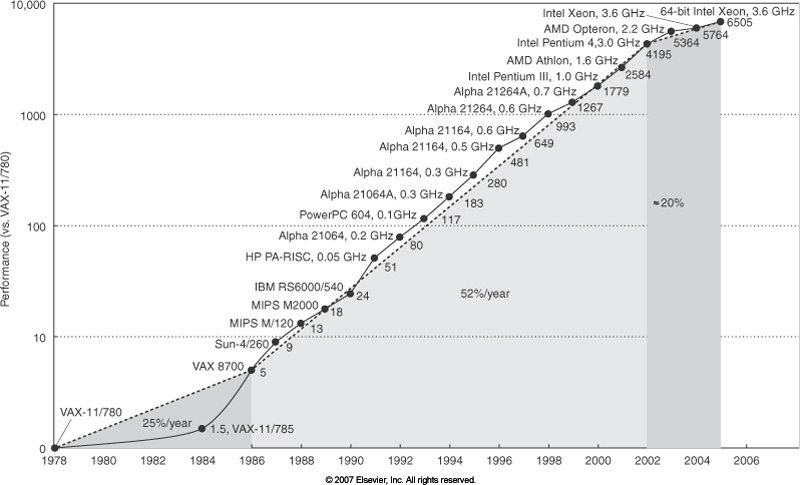
\includegraphics[width=160mm, height=100mm]{images/computing-power-patterson.jpg}
\caption{Growth in processor performance since the mid-1980s. Copyright 2009 Elsevier. All Rights Reserved. \label{overflow}}
\end{center}
\end{figure}

As we can see, prior to the mid-1980s processor performance growth averaged about 25\% per year and this increased to about 52\% until 2002. This increase of almost 25\% has been achieved through Instruction Level Parallelism (ILP). However those gains were expunged and since 2002, it has slowed to about 20\% per year. Also, the continuous increase of clock speed has led to a bottleneck regarding the produced power from computing systems. In the figure 2.2, we can see a graph containing the relationship between the clock speed of a intel i7-2600K processor and the produced power.

\begin{figure}[ht!]
\begin{center}
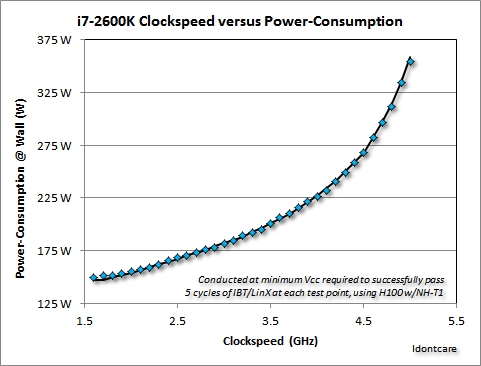
\includegraphics[width=130mm,height=70mm]{images/clock-vs-power.png}
\caption{Graph of Clockspeed versus Power Consumption \label{overflow}}
\end{center}
\end{figure}

From the previous graph, it is evident that the benefits of the increase in clock speed could not be easily reaped, since there are limitation in the maximum power and heat that a computing system can produce. The previous phenomenon can be explained by Moore's law, since much of the increase of transistors was the reason why a great percentage of the power that was produced was returned to the system due to leakage currents and defects. With leakage power dominating, power consumption is roughly proportional to transistor count. According to Pollack's Law, processor performance grows proportionally to the square root of the area. Completing the necessary calculations as we can see in figure 2.3, this led to a shift to multiprocessing systems.

\begin{figure}[ht!]
\begin{center}
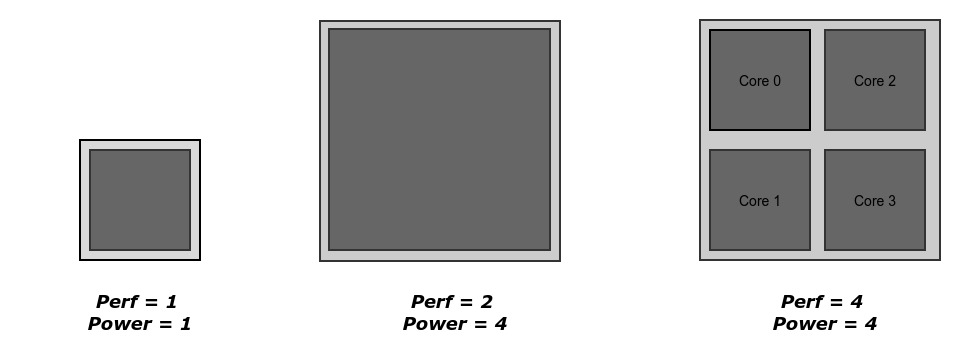
\includegraphics[width=150mm, height=50mm]{images/multicore.jpg}
\caption{Performance comparison between single-core and multicore systems \label{overflow}}
\end{center}
\end{figure}

\subsection{Memory Speed Progress}

According to Moore's Law, there is also an observation that there is a difference between the progress in CPU performance and the progress in Memory performance and this difference is constantly growing by 50\% every year. This can also be seen in figure 2.4. This difference imposes a really hard problem in the attempts to improve the infrastructure of computing systems. The processing power of computing systems evolves, but the memory speed increases slowly. This fact creates a severe bottleneck in the performance of computing systems, since applications waste a great part of their execution time by waiting for requests to memory.

\begin{figure}[ht!]
\begin{center}
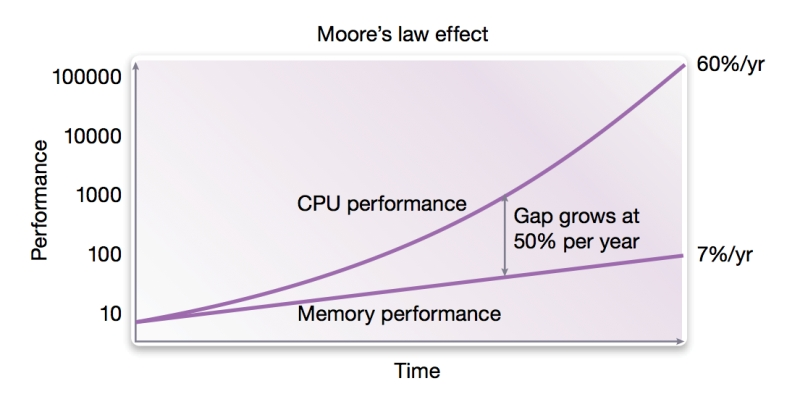
\includegraphics[width=150mm, height=70mm]{images/memory-wall.jpg}
\caption{Difference between processor performance progress and memory speed progress \label{overflow}}
\end{center}
\end{figure}

As also stated in "Hitting the Memory Wall : Implications of the obvious" \cite{reference5}, this difference is already an issue, but it will be a much bigger one in in the future. In this paper, the author has attempted to exclude the implications of the cache memories in this consideration by assuming a perfect performance in the cache hierarchy. The author admits that its own prediction regarding the cessation of the rate of improvements in computer performance might not be so accurate, but she insists that we have to start thinking out of the box in order to find a solution to this complex problem. It is stated that the most convenient resolution to the problem would be the discovery of a cool, dense memory technology whose speed scales with that of processors. However, since this type of technology is not easily conceived, we are currently trying to find workaround solutions to temporarily decrease the impact of this issue to computers performance.

\section{Parallel Computing}

The predominance of multicore systems, as explained before, has created a need for new software capable to leverage the benefits of those computing systems. The concepts of Parallel Programming and Multithreaded Programming emerged to satisfy this need. Multithreaded Programming allows software engineers to create applications separated in multiple threads, that can occupy the different cores of the computing system, thus allowing the application to be more responsive and complete faster. Most programming languages provide the necessary framework to create an application that can be created with multithreaded organisation, so that it can take advantage of multicore systems. However, in most cases the programmer has to be responsible for the switching between threads and their communication, so that there are no errors in applications. Parallel Programming is a model for creating parallel programs which can be compiled and executed in parallel. Depending on the used programming language, the programmer can either choose to let the operating system allocate resources to different instances or otherwise pre-define the way the resources will be allocated to each thread and the way multiple threads will communicate with each other. In the following parts, we will analyse the different forms of parallel programming and the implications of each one to the performance of the computing system.

\subsection{Taxonomy}

The models of parallel programming can be classified by using 2 different criterias: the process interaction and the problem decomposition.

\subsubsection{Process Interaction}

Process interaction involves the mechanisms by which the various instances of an application can communicate with each other. There are 3 basic forms of interaction : shared memory, message passing and implicit. \\

\textbf{\emph{Shared Memory}} is a model of parallel programming used in architectures, where all the processors can access a globally shared memory. Shared Memory architectures can use either Uniform Memory Access (UMA), where all the processors share the physical memory uniformly, or Non-Uniform Memory Access (NUMA), where memory access depends on the distance between each processor and the physical memory. In this model, parallel tasks share a global address space which they read and write to asynchronously. This requires protection mechanisms, such as locks, semaphores and monitors to control concurrent access.

\textbf{\emph{Message Passing}} is a concept from computer science that is used extensively in the design and implementation of modern software applications, where a process sends a message to another process and relies to the second one to select and invoke the actual code to run. In a message passing model, parallel tasks exchange data through passing message to one another. This communication can be either asynchronous or synchronous. The message passing model is used in architectures with distributed physical memory to each core.

\textbf{\emph{Implicit parallelism}} is a model, where the programmer has no vision of the process interaction, since the compiler or interpreter automatically exploits the parallelism inherent to the computations expressed by some of each language's constructs. So, the programmer does not need to worry about task division or process communication, resulting in a significant improved programmer productivity. However, this model is applicable only with domain-specific languages where the concurrency with a problem can be more prescribed.

\subsubsection{Problem Decomposition}

Problem Decomposition involves the structure around which the algorithm for the solution of a problem is constructed. This classification can also be referred as algorithmic skeletons. There are 3 basic forms of problem decomposition : task parallelism and data parallelism. \\

\textbf{\emph{Task Parallelism}} focuses on matching each process with a specific task and distributing those processes across different parallel computing nodes. These processes will often be behaviourally distinct, which emphasizes the need for communication.

\textbf{\emph{Data Parallelism}} on the other hand focuses on distributing the data across different parallel computing nodes. The operations that are performed in the given data set are usually structured in an array. A set of tasks will operate on this data, but independently on separate partitions. In a shared memory system, the data will be accessible to anybody, while in a distributed memory system it will be divided between processes. \\

Actually, most real programs fall somewhere between task parallelism and data parallelism as far as this classification is concerned. As it became obvious from the previous categorization, there were 2 basic architectures around the parallel programming models. The first architecture that came up was the Symmetric Multiprocessors (SMPs), where there were multiple CPUs with one core per CPU. All the caches were private to each CPU and the communication was conducted through the main memory. However, this architecture was not so efficient, because the phenomenon of false sharing was leading to costly memory accesses. So, it has been increasingly replaced by Chip Multiprocessors (CMPs), where there are multiple CPU cores on one integrated circuit. Each core has its own private caches and the last-level caches are shared among the cores of a chip. In this architecture, false sharing impact is limited by the shared last-level caches.

\subsection{MESI Protocol}

The predominance of CMPs was the main cause of a new issue called Memory Coherence. This issue affects the computing systems, where 2 or more processors share a common area of memory, as it is the case with the last-level caches of CMPs. More specifically, Cache Coherence is the consistency of shared resource data that ends up stored in multiple local caches. Coherence, for instance, defines the behavior of read and writes to the same shared last-level cache by different cores. The change of the architectures required a corresponding adaptation in the way the operating system would treat those shared resources. Among many protocols that were suggested as Cache Coherence protocols, the most widespread is the MESI protocol, which supports write-back cache. We will try to give a brief analysis of this protocol, since it is mainly involved in the prediction model of the suggested scheduler. \\

In this protocol, every cache line is marked with one of the 4 following states (using 2 bits) : \\

\textbf{\emph{Modified}} : the cache line is present only in the current cache and it is dirty, which means it has been modified from the value in main memory. The cache is required to write the modified value back to the main memory at some time in the future, before permitting any other read of the (no longer valid) main memory state. This operation, called write-back, changes the line state to Exclusive.

\textbf{\emph{Exclusive}} : the cache line is present only in the current cache, but it is clean, which means it matches main memory. It may be changed to the Shared state at any time, in response to a read request. Alternatively, it may be changed to the Modified state when writing to it.

\textbf{\emph{Shared}} : this cache line may be stored in other caches of the machine and it is clean. The line may be discarded at any time.

\textbf{\emph{Invalid}} : this cache line is invalid (unused).

A Read For Ownership (RFO) request is an operation in cache coherency protocols that combines a read and an invalidate broadcast. The operation is issued by the processor trying to write into a cache line that is either in the Shared state or in the Invalid state of the MESI protocol. The operation causes all other processors to set the state of this line to Invalid. A read for ownership transaction is a read operation with intent to write to that memory address. Therefore this operation is exclusive. It brings data to the cache and invalidates all other processor caches which hold this memory line.

\subsection{Challenges in Multicore Systems}

As a conclusion, during the last decades there has been a turn to multicore systems, since it is claimed that they can provide higher degrees of performance. However, it is indisputable that those new hardware architectures have imposed new problems that have to be resolved if multicore systems are to reach their full potential. The main challenges that we have to face in multicore systems are 2. The first one is the memory bandwidth limitation in systems, in which the number of cores is significantly increased up to an extent, where important contention is observed in the shared memory bus during input or output of programs. The second challenge is the communication between different processes that run in cores of the same chip. In cases of strange data-sharing patterns, this can lead to continuous invalidation between different cores, which is stated as cache thrashing. In both cases, the contention in system resources is the crucial factor that has a major impact in the performance of the system. This can not be prevented in application-level. It can only be faced in a lower level, where we could manage the combination of applications, so that contention bottlenecks are avoided as much as possible. This is the reason why a great part of research has been devoted around contention-aware scheduling solutions, since they present really promising results regarding the overall performance of the computing system.

\section{Scheduling}

In computing, scheduling is the component of the operating system that allows threads, processes or data flows to have access to system resources, such as processing time and memory bandwidth. This is usually done to load balance and share system resources or achieve a target quality of service. The need for a scheduling algorithm arises from the requirement for most modern systems to perform multitasking (executing more than one process at a time) and multiplexing (transmit multiple data streams simultaneously across a single physical channel).

\subsection{Operating Systems Scheduling}

The basic characteristics for a scheduler are the following :
\begin{itemize}
	\item \textbf{\emph{Throughput}}, the total number of processes that complete their execution per time unit
	\item \textbf{\emph{Latency}}, which is divided into
		\begin{itemize}
			\item \textbf{\emph{Turnaround time}}, which is the total time between submissions of a process and its completion
			\item \textbf{\emph{Response time}}, which is the time from submission of a process until the first time it is scheduled.
		\end{itemize}
	\item \textbf{\emph{Fairness}}, which is the attemt to give equal CPU time to each process or more generally appropriate times according to each process' priority and workload
	\item \textbf{\emph{Waiting time}}, which is the time the process remains in the ready queue
\end{itemize}

However, these goals often conflict, thus a scheduler will implement a suitable compromise. For instance, the target of throughput can be controversial to that of low latency. So, focus is given to any of the characteristics mentioned before, depending upon the user's needs and objectives. As a result, the scheduler is a component of the operating system that selects the next jobs to be admitted into the system and the next process to execute. \\

Operating systems may feature up to 3 distinct types of scheduler : 
\begin{itemize}
	\item \textbf{\emph{Long-term scheduling}} or admission scheduler decides which jobs are to be admitted to the ready queue (in the main memory). When an attempt is made to execute its admission to the set of currently executing processes is either authorized or delayed by the long-term scheduler. So, this scheduler decides what processes are to run on a system and the degree of concurrency to be supported at any time, which means whether a high or low amount of processes are to be executed concurrently, and how the split between I/O bound and CPU bound processes is to be handled. The long term scheduler is responsible for controlling the degree of multiprogramming. It is mainly used in large-scale systems, such as batch processing systems, computer clusters, supercomputers and render farms.
	\item \textbf{\emph{Medium-term scheduling}} temporarily removes processes from main memory and places them on secondary memory, like disk drive or vice versa. This process is referred to as 'swapping out' or 'swapping in' correspondingly. The medium-term scheduler may decide to swap out a process which is waiting response from the memory for a long time, a process that has low priority or a process that is page faulting frequently. The scheduler will swap the process back in, when the process has been unblocked and is no longer waiting for a resource. In systems that support mapping virtual address space to storage other than the swap file, the medium-term scheduler may actually perform the role of the long-term scheduler.
	\item \textbf{\emph{Short-term scheduling}}, also known as the CPU scheduler, decides which of the ready, in memory processes are to be executed after a clock interrupt, an I/O interrupt, an operating system call or another form of signal. Thus, the short-term scheduler makes scheduling decisions much more frequently than the long-term or the medium-term schedulers. It will have to make a scheduling decision at least after every time quantum, which are really short periods. This scheduler can either be preemptive or non-preemptive. Preemptive schedulers are capable of forcibly removing processes from a CPU when the time quantum of their execution has finished. Non-preemptive schedulers, also known as 'cooperative' or 'voluntary', is unable to force processes off the CPU. A preemptive scheduler relies upon a programmable interval timer which invokes an interrupt handler that runs in kernel mode and implements the scheduling function. It can also be referred to as process scheduler.
\end{itemize}

\subsection{Major Scheduling disciplines}

Scheduling disciplines are generic algorithms used for distributing resources among parties which simultaneously and asynchronously require them. Scheduling disciplines can be used in routers as well as in operating systems, disk drives, printers etc. The main purpose of scheduling disciplines are to prevent resource starvation and to guarantee fairness amongst the parties utilising the resources. Scheduling deals with the problem of deciding which of the outstanding requests is to be allocated resources. Each discipline uses different criteria to explain its decisions. The main scheduling disciplines are the following : \\

\begin{itemize}
\item \textbf{\emph{First Come First Served}} (FCFS) is the simplest scheduling algorithm. It simply queues processes in the order that they arrive in the ready queue. This kind of scheduling is non-preemptive, so the processes will start start and finish in the order that they arrive in scheduler queue. Since context switches occur only upon process termination and no reorganization of the queue is required, the scheduling overhead is minimal. The total throughput can be low, since some processes can hold the CPU even when they are blocked. Turnaround time, waiting time and response time can also be high for the same reason. The systems faces trouble meeting process deadlines, since there is no prioritisation in processes. However, the lack of prioritization means that as long as every process eventually completes, there is no starvation. \\

\item \textbf{\emph{Shortest Job First}} (SJF) is a discipline, where processes with the least estimated processing time are the next to be scheduled. First of all, this requires advanced knowledge or estimations about the time required for a process to complete. This scheduling is preemptive. Thus, if a shorter process arives during another process' execution, the currently running process will be interrupted and the arrived process will be executed. This creates excess overhead through additional context switching. Waiting time and response time increase as the process's computational requirements increase.  Overall waiting time is smaller than FIFO, since no process has to wait for the termination of the longest process. Besides the additional infrastructure needed for this scheduling discipline, the main problem is the possibility of starvation of long processes, if short processes arrive continuously in the queue. \\

\item \textbf{\emph{Fixed priority preemptive scheduling}}, where the operating system assigns a fixed priority rank to every process and the scheduler arranges the processes in the ready queue in order of their priority. Since this scheduling discipline is preemptive, lower-priority processes get interrupted by incoming higher-priority processes. The scheduling overhead is not minimal, nor it is significant. If the number of rankings is limited, it can be characterized as a collection of FIFO queues, one for each priority ranking. Processes in lower-priority queues are selected only when all of the higher-priority queues are empty. Deadlines can be met by giving processes with deadlines a higher priority. Starvation is possible, but it can be avoided, if aging is implemented so that processes do not stay in the same priority queue forever. \\

\item \textbf{\emph{Round Robin scheduling}} (RR) assigns a fixed time unit per process (defined as time quantum), and cycles through them. It involves extensive overhead, especially with a small time unit. It has a balanced throughput between  FCFS and SJF. Short processes are completed faster than in FCFS and long processes are completed faster than in SJF. It has a good average response time and the waiting time is dependent on number of processes and not on average process duration. Deadlines are rarely met in RR Scheduling, because of high waiting times. Starvation can never occur, since no priority is given. There is also significant overhead in the context switch between processes when the time quantum finishes, especially if its duration is really short. \\
\end{itemize}

In the following sections, we will give a brief description of the CFS scheduler of Linux and other state-of-the-art contention-aware schedulers, since our proposed scheduler will be finally compared with these schedulers.

\subsection{Linux Scheduler - CFS}

The Completely Fair Scheduler (CFS) is a process scheduler which was merged into the 2.6.23 release of the Linux kernel and is the default scheduler. We could say that it is a combination of round robin and fixed priority preemptive scheduling. It handles CPU resource allocation for executing processes, and aims to maximize overall CPU utilization while also maximizing interactive performance. In contrast to the previous O(1) scheduler used in older Linux 2.6 kernels, the CFS scheduler implementation is not based on run queues. Instead, a red-black tree implements a "timeline" of future task execution. Additionally, the scheduler uses nanosecond granularity accounting, the atomic units by which an individual process' share of the CPU was allocated (thus making redundant the previous notion of timeslices). This precise knowledge also means that no specific heuristics are required to determine the interactivity of a process, for example. Like the old O(1) scheduler, CFS uses a concept called "sleeper fairness", which considers sleeping or waiting tasks equivalent to those on the runqueue. This means that interactive tasks which spend most of their time waiting for user input or other events get a comparable share of CPU time when they need it. \\

The data structure used for the scheduling algorithm is a red-black tree in which nodes are scheduler specific structures (called sched\_entity). A red black tree is a data structure which is a type of a self-balancing binary search tree. Balance is preserved by colouring the nodes with 2 colors (black and red) according to some properties, which define how unbalanced the tree can become in the worst case. Each time the tree is modified, the new tree is subsequently rearranged and repainted to restore coloring properties. The properties are designed in such a way that this rearranging and recoloring can be performed efficiently. The balancing of the tree is not perfect, but it guarantees searching in $O(logn)$ time, where n is the total number of elements in the tree. The insertion and deletion operations are also performed in $O(logn)$ time. Tracking the color of each node requires only 1 bit of information per node because there are only two colors. In CFS, the nodes of the red-black tree represent the processes. These nodes are indexed by processor execution time in nanoseconds. A maximum execution time is also calculated for each process. This time is based upon the idea that an "ideal processor" would equally share processing power amongst all processes. Thus, the maximum execution time is the time the process has been waiting to run, divided by the total number of processes, or in other words, the maximum execution time is the time the process would have expected to run on an "ideal processor". \\

When the scheduler is invoked to run a new process, the workflow of the scheduler is the following :
\begin{enumerate}
    \item The left most node of the scheduling tree is retrieved by the scheduler (as it will have the lowest spent execution time) and scheduled for execution.
    \item If the process simply completes execution, it is removed from the system and scheduling tree.
    \item If the process reaches its maximum execution time or is otherwise stopped (voluntarily or via interrupt) it is reinserted into the scheduling tree based on its new spent execution time.
    \item The new left-most node is selected from the tree, repeating the iteration.
\end{enumerate}

If the process spends a lot of its time sleeping, then its spent time value is low and it automatically gets the priority boost when it finally needs it. Hence those kind of tasks do not get less processor time than the tasks that are constantly running.

\subsection{Contention-Aware schedulers}

A crucial factor that is somewhat ignored in the implementation of the Completely Fair Scheduler is the fact that the different cores of a multicore system are directly dependent. CFS treats applications simply as single-threaded applications and cores as black boxes, where there is not interaction between different cores. However, this is not the truth. As it became evident in the previous analysis, there are multiple bottlenecks present in multicore systems. The impact of those bottlenecks is highly influenced by the profile of the applications and the way they interact with each other. For instance, if 2 applications that present similar data-use patterns are scheduled in cores of the same chip, then each one will invalidate the data of the other application due to Cache Coherence protocols, such as MESI protocol described before. Likewise, if 2 applications that use extensively the memory link are scheduled in cores of the same chip, then they will end up sharing the available memory bandwith and this will lead to serious performance degradation. However, if we crossed the pairs scheduling one application using the memory with one application using the last-level cache, then we would have managed to decrease significantly the competition between the 2 application and as well as ease the performance degradation. As a result, CFS scheduler would be drastically improved, if it was evolved into a contention-aware scheduler that would be able to detect those bottlenecks and handle them. An ideal contention-aware scheduler would have to be capable to characterize the applications in order to estimate the place of contention and then schedule the applications in suitable combinations, so that competition in system resources between application is minimized. \\

The research about contention-aware schedulers has progressed with big steps. A lot of contention-aware schedulers have been proposed both for UMA and NUMA systems with really promising results. For UMA systems, some of the best suggested contention-aware schedulers are :
\begin{itemize}
    \item OBS-X scheduling policy based on OS Dynamic Observations \cite{reference21}: this scheduling policy uses observations of each task's cache usage in order to distribute cache-heavy threads throughout the system, aiming to spread out cache load. When a new task is created, OBS-X looks for the LLC group with the smallest cache load, and places the new task in this group. this scheduling policy was only compared with the Linux default scheduler and it presented overall speedup increase up to 4.6\%. \\
    \item Vector Balancing Scheduling policy \cite{reference22}: this policy reduces contention by migrating tasks, led by the information of task activity vector, that represents the utilization of chip resources caused by tasks. The proposed scheduling policy avoids contention for resources by co-scheduling tasks with different characteristics. One weakness of this paper is that they used exclusively compute-intensive tasks and this limits the space where the Vector Balancing can be applied successfully. \\
    \item Distributed Intensity Online scheduler (DIO) \cite{reference23}: this scheduler continuously monitors the miss rates of applications, since it is argued that this is the best contention predictor, then finds the best performance case and separates threads. It obtains the miss rates of applications dynamically online via performance counters. This makes DIO more attractive since the stack distance profiles, which require extra work to obtain online, are not required. It was compared to the default Linux scheduler and increased the total performance by 13\%. An adapted version of this scheduling policy has also been implemented for NUMA systems, called DINO. DINO tries to migrate threads in the same memory areas when possible. It uses the same heuristis with DIO and divides applications in categories depending on the number of LLC misses they have per 1.000 instructions. \\
    \item Symbiotic JobScheduling \cite{reference19} : this scheduler combines an overhead-free sample phase which collects information about various possible schedules, and a symbiosis phase which uses that information to predict which schedule will provide the best performance. However, it required a sampling phase in which, the workload is not scheduled optimally. \\
    \item AMPS scheduler \cite{reference24} : this scheduling is implemented both for SMPs and NUMA-style performace assymetric architectures. AMPS contains the following components : assymetry-aware load-balancing, that balances threads to cores in proportion with their computing power and faster core-first scheduling, that controls thread migrations based on predictions of their overhead. However, AMPS uses thread-independent policies, which schedule threads independently regardless of application types and dependencies, which is a rather significant weakness. \\
    \item Framework for Adaptive Contention-Aware Thread Migrations (FACT) \cite{reference20} : this approach monitors some performance indicators lively during the execution, predicts the bottlenecks and makes adaptations to the scheduling in order to avoid contention and improve overall performance. In the implementation of FACT, a variety of statistical models were used, such as linear regression models, fuzzy rule-based models, decision-tree models, K-nearest neighbor models. It proved to be slightly better than DI, but it relies on supervised learning and targeted the same problem from a whole different view. \\
\end{itemize}

As a conclusion, there are multiple contention-aware schedulers suggested from previous research. The majority of those schedulers have been compared to the default Linux scheduler, so as to ensure that the benefits from transition to contention-aware scheduling will be significant. However, there is not so much comparison between proposed contention-aware schedulers. Furthermore, all those schedulers are compared with the Linux default scheduler solely as far as overall performance is concerned, leaving outside the consideration the degree of fairness imposed by the scheduler. Since both throughput and fairness are significant properties of a scheduling policy, we will make comparisons using both criteria. \\

Our scheduler takes into consideration all kinds of applications, ranging from applications that are CPU-bound to applications that stress extensively the main memory. However, we have adjusted all applications so that they have integrated the input data set, in order to avoid I/O actions. This makes the workload not so realistic, but the I/O delays is an issue that can be resolved independently and is not included in systems resource contention. The miss rate was used as heuristic at OBS-X scheduler, Vector Balancing Scheduler, DIO and FACT. Moreover, the memory link usage was used as heuristic for detecting resources contention at Vector Balancing Scheduler, Symbiotic scheduling and FACT. It is consequently obvious that those 2 measures are the most useful heuristics regarding system resources contention. For this reason, our scheduler will be compared with the default Linux scheduler and 2 contention-aware schedulers that are derived from the previously mentioned research. Those schedulers are the LLC-MRB and the LBB scheduler. The first one attempts to balance the last-level cache misses in the whole system, while the latter one tries to balance the memory link usage. This is achieved using a queue with all the applications sorted by their LLC misses (or memory bandwidth correspondingly) and the applications are paired suitably, so that applications that present high contention are co-scheduled with applications with low contention. The comparison between our scheduler and the rest will be in terms of fairness and total throughput. 

\section{Experimentation Environment}

The comparison between the different schedulers is performed on an Intel Xeon R CPU E5-4620 Sandy Bridge architecture machine. The architectural details are presented in Table I. All the available hardware prefetchers are enabled whereas Hyperthreading and Turbo Boost are disabled. The platform's kernel was Debian Linux 6.0.6 with kernel 3.7.10.

\begin{table}[h]
\begin{center}
\caption{Sandy Bridge Architecture Details}
\begin{tabular}{ | l | l | }
    \hline
    Cores & 8 \\ \hline
    L1 & \makecell{Data Cache: private, 32KB, 8-way, 64 bytes block size \\ Instruction Cache: private, 32KB, 8-way, 64 bytes block size} \\ \hline
    L2 & private, 256KB, 8-way, 64 bytes block size \\ \hline
    L3 & shared, 16MB, 16-way, 64 bytes block size  \\ \hline
    Memory &  64GB, DDR3, 1333MHz \\ \hline
    OS & Debian Linux 6.0.6 with kernel 3.7.10 \\ \hline
\end{tabular}
\end{center}
\end{table}

The prediction model was tested in the previous platform, but for more complete validation it was also tested in another machine with an AMD Opteron 248 Nehalem architecture. The architectural details of the second machine can be seen in the table 2.

\begin{table}[h]
\begin{center}
\caption{Nehalem Architecture Details}
\begin{tabular}{ | l | l | }
    \hline
    Cores & 4 \\ \hline
    L1 & \makecell{Data Cache: private, 32KB \\ Instruction Cache: private, 32KB} \\ \hline
    L2 & private, 256KB \\ \hline
    L3 & shared, 16MB\  \\ \hline
    Memory &  32GB \\ \hline
    OS & Ubuntu 12.04.2 LTS \\ \hline
\end{tabular}
\end{center}
\end{table}

A diagram of the Sandy Bridge architecture that was mainly used for the design and verification of the prediction model, as well as for the implementation and testing of the scheduling algorithm can be seen in the Figure 2.5 \\


\begin{figure}[ht!]
\begin{center}
\hspace*{-1cm}
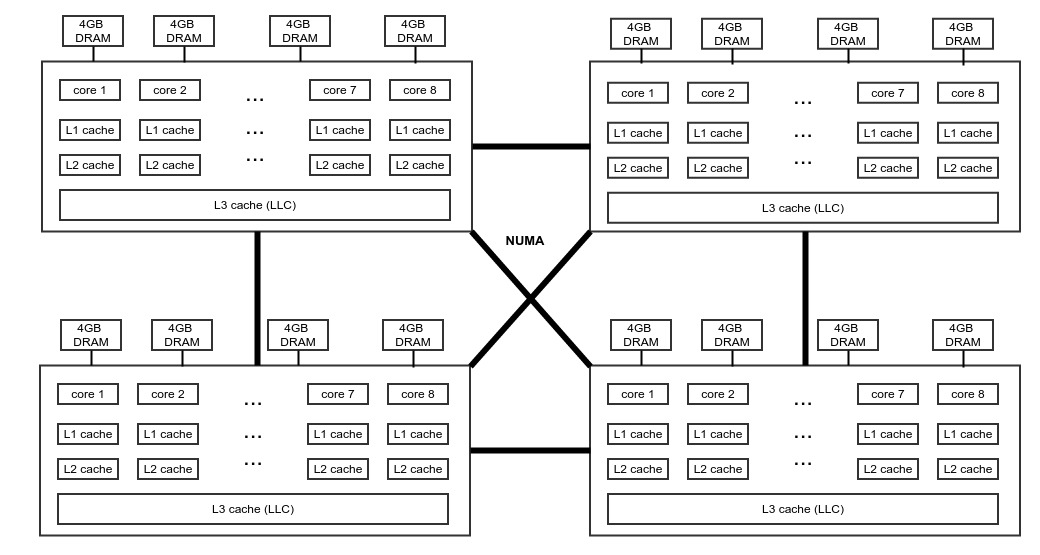
\includegraphics[width=175mm, height=210mm]{images/sandman-architecture.jpg}
\caption{Sandy Bridge architecture  \label{overflow}}
\end{center}
\end{figure}

The various counters that have been used for the investigation and verification of the classification scheme and the prediction model can be seen in table 2.3. This table contains the Intel hexadecimal codes for both architectures Nehalem and Sandy Bridge. We remind that the Nehalem architecture was used only in the step of verification of the prediction model.


\begin{table}[!h]
\centering
\caption{Intel Hardware Performance Counters used}
\begin{tabular}{| c | c | c | c | c |}
\toprule
{}  &  \multicolumn{2}{| c |}{Sandy Bridge} & \multicolumn{2}{| c |}{Nehalem}\\
\midrule
Counter Name   & Event Num.   & Umask    & Event Num.   & Umask\\
L1 lines allocated in Modified  &  0xD2 & 0x0F   & 0x51  & 0x02\\
L1 lines evicted in Modified due to hitM or dirty &  0x51 & 0x08   & 0x51  & 0x08 \\
L1 lines evicted in Modified due to replacement  &  0x51 & 0x51   & 0x51  & 0x04 \\
L1 -> L2 writebacks  &  0xfo & 0x10   & 0x28  & 0x0F \\
L2 cache lines allocated in Invalid  &  0xF1 & 0x01   & --  & -- \\
L2 cache lines allocated in Shared  &  0xF1 & 0x02   & 0xF1  & 0x02 \\
L2 cache lines allocated in Exclusive  &  0xF1 & 0x04   & 0xF1  & 0x04 \\
RFO requests that access L2 cache  &  0xF0 & 0x02   & 0x24  & 0x0C \\
Dirty L2 cache lines evicted  &  0xf2 & 0x05   & 0xF2  & 0x02 \\
Clean L2 cache lines evicted by prefetcher  &  0xF2 & 0x0a   & 0xF2  & 0x04 \\
Snoop invaliations of Modified line  &  0x22 & 0x50   & --  & --\\
L3 lines allocated in Exclusive  &  0x0A & 0x02   & 0x0A  & 0x02 \\
L3 lines allocated in Shared  &  0x0A & 0x04   & 0x0A  & 0x04 \\
LLC snoops invalidations due to memory requests  &  0x34 & 0x4F   & --  & --\\
Micro-operations retired  & 0xC2 & 0x01 & 0xC2 & 0x01 \\
Memory micro-operations retired & 0xD0 & 0x81 & 0xC2 & 0x81 \\
\bottomrule
\end{tabular}
\end{table}

The suggested scheduler is made of 3 components : the classification scheme, the prediction model and the scheduling algorithm. Each one of the following chapters analyses one component of the scheduler. \\


\chapter{Classification Scheme}

In this chapter, we will cover the classification scheme used by our scheduler.

\section{Previous Research}

All contention-aware schedulers presented in previous research rely on an application classification scheme that predicts application interference under a co-execution scenario. The accuracy of the classification scheme in the prediction of application co-execution penalties is one of the most critical factors for a co-scheduling framework. Cache utilization patterns, LLC miss rate, memory link bandwidth and sensitivity have been proposed towards this direction. However, as these schemes capture application activity in a limited part of the architecture, i.e. either memory link or last level cache (LLC), they fail to provide a more complete picture of the resources candidate to suffer from contention. This scheduler contains a classification scheme that attempts to take into consideration all possible places of contention in system's architecture. In this way, it can include a different heuristic for each part of the architecture and take into account all the different classes of applications. An attempt is made to cover the entire memory hierarchy from main memory down to the private caches and even the computing cores. This information is utilized to understand application behavior and predict interference problems.

The most dominant classification schemes of previous research are the color classes \cite{reference16} and the animal classes \cite{reference15}. The color classification categorizes applications into one of 4 colors, according to the observed performance degradation when running an program using only a 1MB L2 cache compared to the baseline configuration with 4MB. Any program with greater than 20\% slowdown was classified as Red and greater than 5\% slowdown (but less than 20\%) as Yellow. Out of the remaining programs with less than or equal to 5\% slowdown, the program is classified as Green if the total number of L2 accesses is greater than or equal to 14 misses per thousand cycles, otherwise the program is in the Black category. While Lin et al.’s color-based classification scheme may be useful for workload creation, it cannot be easily used for dynamic, on-the-fly classification of program behavior. In particular, computing the performance slowdown would require simultaneously running two copies of the program on two cores, each with their own dedicated L2 caches. \\


. The animal classification divides the applications into 4 classes : turtles, sheep, rabbits and devils. Turtles do not make rare use of the shared last-level cache, possibly due to small working data sets. Sheeps are applications that are not sensitive to the number of ways allocated to them, so they can exhibit high LLC usage even with a few ways allocated. Rabbits are very sensitive about the number of ways allocated to them. Devils access the last-level cache frequently, but still have very high miss rates. This classification aimed to better identify cache-sharing behaviors and more accurately predict when cache partitioning will be useful. For processors without some form of dynamic cache management/partitioning, one can provide feedback back to the operating system so that the process scheduler can attempt to avoid co-scheduling incompatible animal types, which means it could be used as classification scheme for our approach. However, the animalistic classification does not build a solid theoretical explanation between the various parts of the memory hierarchy and the different classes, as it is the case with our classification scheme

\section{Application classes}

Our classification scheme is inspired by previous research \cite{reference1} and distinguishes between 5 application classes, where the names of the classes are indicative of the parts of the memory that are stressed : 
\begin{itemize}
    \item memory link intensive applications, that exhibit high memory bandwidth
    \item applications that have significant activity both on the memory link and the last-level shared cache
    \item cache intensive applications, that exhibit activity mainly in the last-level cache
    \item cache intensive applications, that exhibit activity in highest level private caches and when competing ending up using last-level cache but not to a extended degree
    \item applications that exhibit no significant activity on the shared resources of the system and are limited to private caches and cores
\end{itemize}
It is now visible that our classification scheme directly bonds the different parts of the memory hierarchy to the different application classes. Interactions between applications from various classes are adequately predictable to support an efficient scheduling mechanism. In the following paragraphs, each application class is described further. \\

\textbf{\emph{Class L}} : Applications with very intense pressure on the memory link, consuming a high percentage of its bandwidth. This class typically includes applications that exhibit one or more of the following characteristics: they perform streaming memory accesses on data sets that largely exceed the size of the LLC, have either no reuse or large reuse distances, perform rather lightweight computations on the data fetched. To reach this high level of memory link bandwidth consumption, members of this class heavily involve the hardware prefetcher in their execution. Although they fetch data on the entire space of the LLC due their streaming nature, they do not actually reuse them either because their access pattern does not recur to the same data, or because they have been swept out of the cache. \\ 

\begin{figure}[ht!]
\begin{center}
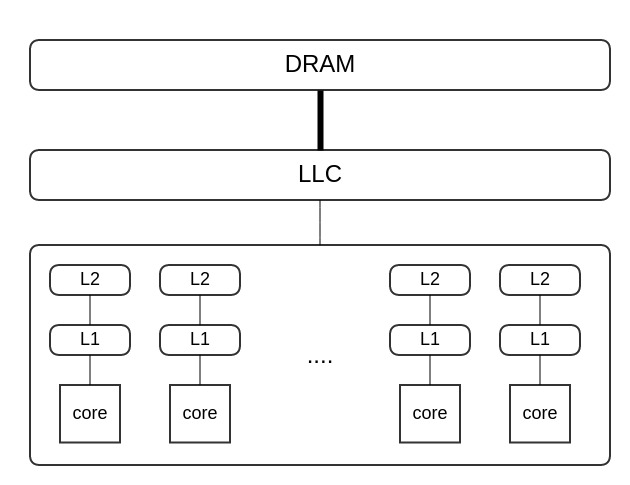
\includegraphics[width=100mm, height=70mm]{images/category_L.jpg}
\caption{Class L applications \label{overflow}}
\end{center}
\end{figure}

\textbf{\emph{Class LC applications}} : Applications with substantial pressure on the memory link and also high activity on the shared LLC. This is a wide class including applications with streaming access and heavy computations on the data fetched, or a combination of main memory access and LLC data reuse. The exact level of memory bandwidth consumption and data reuse on the LLC may significantly differentiate execution behavior within the class. \\\ 

\begin{figure}[ht!]
\begin{center}
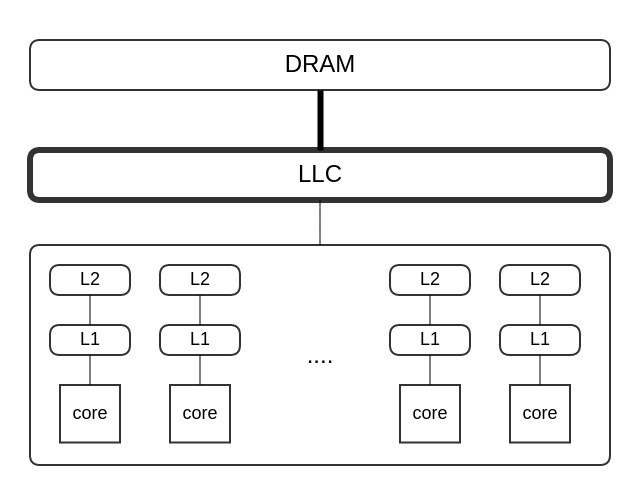
\includegraphics[width=100mm, height=70mm]{images/category_LC.jpg}
\caption{Class LC applications \label{overflow}}
\end{center}
\end{figure}

\textbf{\emph{Class C}} : Applications with heavy activity on the shared LLC. This class includes applications with varying characteristics, such as those that operate on small data sets with heavy reuse, optimized code for the LLC (e.g. via cache blocking with a block size fitting the LLC), or latency-bound applications that make irregular data accesses and benefit a lot from LLC hits. \\ 

\begin{figure}[ht!]
\begin{center}
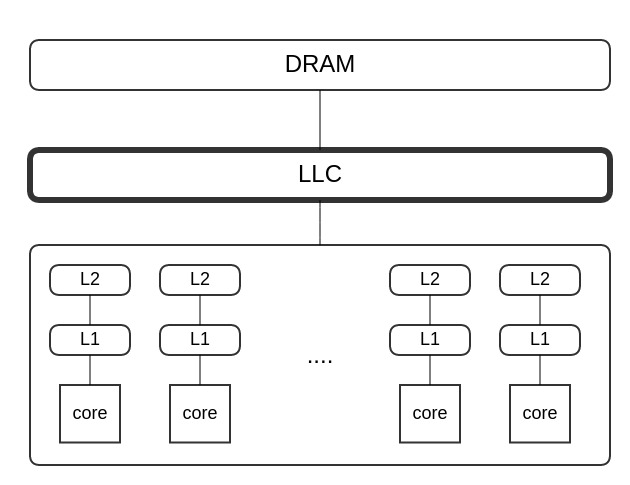
\includegraphics[width=100mm, height=70mm]{images/category_C.jpg}
\caption{Class C applications \label{overflow}}
\end{center}
\end{figure}

\textbf{\emph{Class C+}} : Applications with focused activity on the highest level private caches (L2 cache). In fact, it is a subcategory of class C applications. If executed without major contention in resources, those applications' activity is restricted in private cache. However, if executed with other applications exhibiting significant activity in L2 cache (e.g. with another C+ application), the overall contention will oblige the C+ application to increase the last-level cache usage. \\ 

\begin{figure}[ht!]
\begin{center}
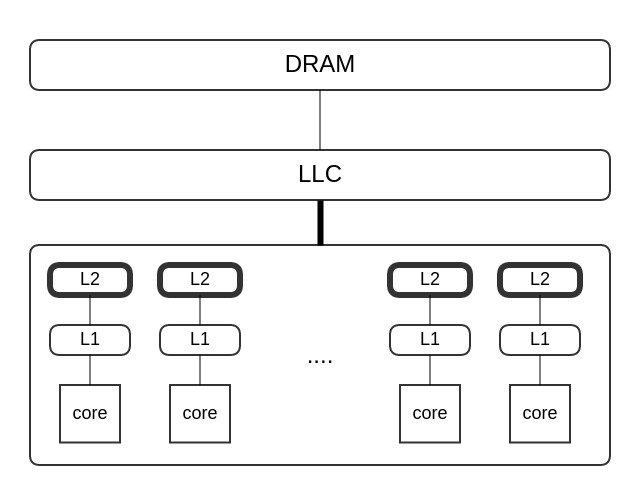
\includegraphics[width=100mm, height=70mm]{images/category_C+.jpg}
\caption{Class C+ applications \label{overflow}}
\end{center}
\end{figure}

\textbf{\emph{Class N}} : Applications that restrict their activity either to the private part of the memory hierarchy or within the core. The members of this class create no contention to the shared system resources. The class includes applications with heavy computations, very small working sets or optimized data reuse that can be serviced by the private caches. \\ 

\begin{figure}[ht!]
\begin{center}
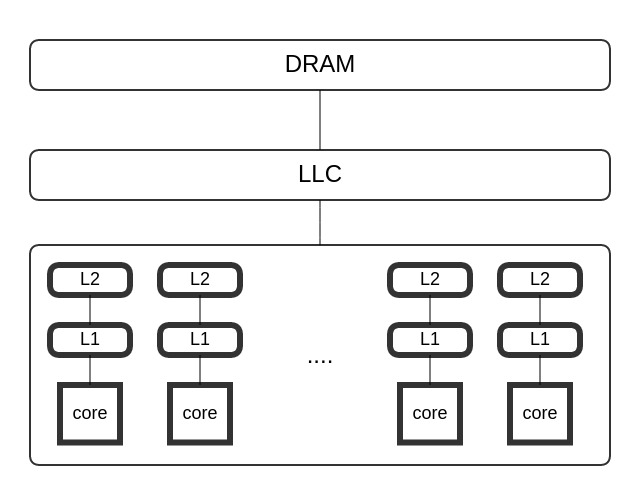
\includegraphics[width=100mm, height=70mm]{images/category_N.jpg}
\caption{Class N applications \label{overflow}}
\end{center}
\end{figure}

Despite the fact that inside each class one may find applications with quite different execution patterns, the classes themselves can be used to capture the big picture of co-execution interference between applications. As it will also be used from the scheduling algorithm in the last step, we need to analyse the interference between each possible combination of applications. In the following we denote as x – y the co-execution of an application from class x with an application from class y. '*' is used as a wildcard for any application class. \\

N - * : This co-execution does not create any interference, since class N applications do not use any shared resource.

L - L : In this co-execution, applications compete for the memory link. The contention pattern in this case indicates that the shared resource which in this case is the memory link bandwidth is divided (not necessarily equally) between the competing applications.

L - C : In this co-execution, applications exhibit activity in different shared resources. However, it will lead to severe performance degradation for C applications with no impact in the performance of L applications. This is due to the fact that the constant delivery of new data from the main memory will invalidate the data of the C application, while L application will not have any problem with those invalidations as it does not use the cache memories.

L - LC : In this co-execution, there will be performance degradation for both applications. However, as described before, LC will face a bigger degradation than L application.

LC - LC : In this co-execution, there will be contention in shared resources, but the contention will be divided between 2 diffent resources (memory link and LLC). For this reason, the interference will be present on both sides but it will be kept in low levels.

LC - C : Similarly, there is some mediocre contention leading to performance degradation. The contention will be more severe for the C application than for the LC application.

C - C : This co-execution is the most difficult to predict, since the impact of the contention will depend upon data access patterns. As it will be described later, the MESI protocol was taken into consideration for this specific co-execution scenario. \\ \\


\section{Decision Tree}

Having defined the application classes, we need a concrete method to perform the classification using runtime statistics. The core idea is to inspect  the data path from main memory down to the core to locate  links with high utilization. We have focused only on the stream  flowing towards the core, as we have empirically found that this direction concentrates the largest portion of contention. A hierarchical approach is followed similarly to the application classes. First of all we examine if the current investigated application consumes a large portion of the system's memory link bandwidth. If this is true, this application belongs to L class. When the memory link utilization is low, activity is restricted from the LLC and downwards. If we are able to measure significant data flow somewhere in the LLC → Core part of the data path, then this is due to data reuse. By locating the reuse region –LLC
or private caches– we can classify applications as C,C+ and N, respectively. \\

In case that low data flow is measured throughout the entire data path, we have identified three application patterns that may exhibit this picture: 1) applications that heavily reuse data on the L1 cache (high activity on the gray arrow of 2) applications that perform computations within the core with minimal data accesses, and 3) memory-latency bound applications that suffer from high LLC miss penalties (and also greatly benefit from LLC hits). We observed that inspecting the application's $mem\_uops/all\_uops$ ratio and IPC suffices to differentiate between C and N classes. \\

Our classification method implements the decision tree shown in Figure 3.6. The L3 reuse has proved to be a better heuristic than memory bandwidth for distinguishing between LC and L classes, since it was combining both memory bandwidth and LLC bandwidth giving a more complete view. For the classification tree, we have used the following relationships and constants:

\begin{align*}
&Memory \ bandwidth = (per\_core\_bw*64)/(10^6) (GB/sec) \\
&LLC \ bandwidth = (l2\_lines\_in*64)/(10^6) (GB/sec) \\
&L2 \ bandwidth = (l1\_lines\_in*64)/(10^6) (GB/sec) \\
&L3 \ reuse = LLC \ bandwidth / Memory \ bandwidth \\
&L2 \ reuse = L2 \ bandwidth / LLC \ bandwidth \\
&g = 0.35 * Maximum Memory Bandwidth \\
&d = 0.25
\end{align*}

%\scalebox{0.51}[0.6]{
\begin{figure}[H]
\begin{forest}
nonterminal/.style={
    symbol,
    rounded corners,
},
for tree = {l=0.5cm}
[Memory Link\\Utilization, align=center, base=bottom
    [L3 reuse < 1.2
        [L, circle, draw]
    ]
    [1.2 < L3 reuse < 8
        [LC, circle, draw]
    ]
    [L3 reuse > 8
        [Cache Links\\Utilization, align=center, base=bottom, grow=270
            [LLC Bandwidth > g\\or\\L2 Bandwidth > g, align=center, base=bottom, grow=250
                [Reuse\\Location, align=center, base=bottom
                    [L3\\(L3 reuse > L2 reuse), align=center, base=bottom
                        [Degree of Reuse
                            [L3 reuse < 100
                                [C, circle, draw]
                            ]
                            [L3 reuse > 100
                                [C+, circle, draw]
                            ]
                        ]
                    ]
                    [L2\\(L3 reuse < L2 reuse), align=center, base=bottom
                        [N, circle, draw]
                    ]
                ]
            ]
            [LLC Bandwidth < g\\and\\L2 Bandwidth < g, align=center, base=bottom
                [Memory-Latency\\bound, align=center, base=bottom
                    [YES\\(mem\_uops uops > d), align=center, base=bottom
                        [C, circle, draw]
                    ]
                    [NO\\(mem\_uops uops < d), align=center, base=bottom
                        [N, circle, draw]
                    ]
                ]
            ]
        ]
    ]
]
\end{forest}
\caption{Classification scheme}
\end{figure}
%}

In order to monitor the applications and acquire their profile, we retrieved hardware performance counters to collect performance data. More specifically, we used UNHLT\_CORE\_CYCLES, INSTR\_RETIRED, LLC\_MISSES, L1D.REPLACEMENT, L2\_LINES.IN, MEM\_UOP\_RETIRED.ALL and UOPS\_RETIRED.ALL. Furthermore, we use OFFCORE\_REQUESTS (0xB7, 0x01; 0xBB, 0x01) together with Intel’s Performance Counter Monitor \cite{reference9} utility to acquire information regarding bandwidth usage. \\

\section{Evaluation and Validation}

The classification scheme is just a component of our scheduler and it is not really valuable to validate it separately, as we are specifically interested in the impact it will have in the overall efficiency of the scheduler. However, this classification scheme is theoretically ground. It has been created using the research done in \cite{reference1} as a starting point. The initial classification scheme of \cite{reference1} has been validated. The process that was followed is the following : a workload of applications belonging to all classes has been created. The applications were initially executed solo and then all the possible combinations of applications were co-executed. The average slowdown of each possible combination of application classes was compared to the initial assumptions of the classification scheme. The slowdowns derived for each possible combination of different application classes from this research can be seen in Figure 3.7 .\\

\begin{figure}[ht!]
\begin{center}
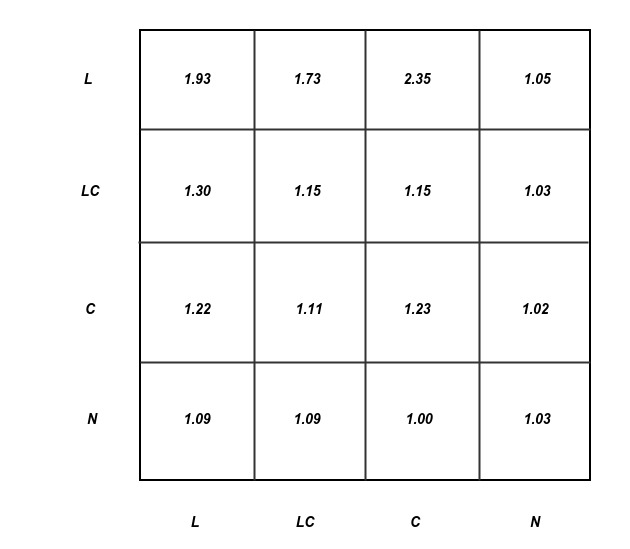
\includegraphics[width=130mm, height=100mm]{images/interference.jpg}
\caption{Average slowdown between different classes \label{overflow}}
\end{center}
\end{figure}

We can observe that, as expected, N applications neither impose nor suffer from interference. C applications, as predicted, experience dramatic slowdowns when co-executed with L applications and in general do not impose severe interference with a few remarkable exceptions. Interestingly, although the LC class may contain a wider variety of activity patterns, their interference behavior is more or less uniform: they suffer more by the co-execution with L applications, and then by the co-execution with applications of the same class. In general, they do not also heavily interfere with C applications. As a result, the assumptions that were initially made are verified.


\chapter{Prediction Model}

The next step after classifying an application is to use our prediction model in order to make an estimation of the maximum resources that can be allocated in an application without provoking resource contention and performance degradation. This is the differentiating factor between our proposed scheduler and the other state-of-the-art contention-aware schedulers. The other schedulers treat applications either as single-threaded applications or as multi-threaded applications, where the resources that will be allocated are in some way predefined. However, this is a big limitation to the benefits we can gain from multicore systems. In an ideal situation, the applications would be handed to the operating system simply as multi-threaded applications and the operating system would allocate the ideal amount of resources to each application in order to achieve the optimum overall performance. In order to make this feasible, the operating system should have a mechanism that would characterize each application and estimate its future performance for different alocations of resources. In this way, the scheduler of the operating system would be capable of taking full advantage of all applications without allowing severe performance degradation due to contention on shared resources. \\ 

This is accomplished through a prediction model. The design of the prediction model was initiated through statistical examination of the correlation between various hardware performance counters (HPCs). There was a statistical correlation between some counters and the scaling of some applications. This was also expected from a theoretical view, since it would be really unreasonable if the contention of the system resources could not be detected through the hardware performance counters. So, after ensuring that there was a statistical correlation between some counters and the scaling of the corresponding applications, we moved on examining specific counters that were relative to the specific part of the memory hiearchy that the contention was present. \\

\section{Theoretical Foundation}

We will present a really brief short introduction to the theoretical aspect of the relationships that will be defined in the next section. As described before, a different counter is expected to be useful for the predictions for each application class. \\

\textbf{\emph{L applications}} - For applications belonging to class L, contention is mainly observed in the memory link, so the memory bandwidth is the crucial factor. The maximum memory bandwidth of the system has to be known. In our case, the maximum memory bandwidth of the system was measured using the stream benchmark \cite{reference7} (executing only the triad version, so that results were not affected). As stated also in the classification scheme, it is assumed that L applications will share the available memory bandwidth almost proportionally. As a result, an L application is expected to stop scaling significantly when the memory bandwidth of the system will be totally consumed. \\

\textbf{\emph{LC applications}} - Applications that belong to this class exhibit significant activity in last-level cache and a less significant activity in memory link. So, we would expect that the measure defining the scaling of an LC application would involve a counter relative to the use of the last-level cache and perhaps a counter that would be relative to the degree in which the application "exits" the last-level cache and requires data from the main memory. \\

\textbf{\emph{C and C+ applications}} - Applications of this class present increased usage of the shared last-level cache and the highest level private cache. The Cache Coherency is expected to be the defining factor regaring the scaling potential of the application. More specifically, we examined the hardware performance counters of the MESI protocol, since we assumed that the data sharing patterns between the applications would define the performance degradation. The data sharing patterns between 2 applications should be derived from MESI-specific counters depicting the currents states of the cache lines. \\

\textbf{\emph{N applications}} - Applications of this class restrict their activity in the low-level private caches and in the cores. As a result, if we allocated more resources to this kind of applications, they should scale almost ideally, since the different threads of the application would not interfere. \\

\section{Linear Regression Model}

We believed that the prediction model could be implemented as linear regression model, since we had previously observed increased correlation coefficients. The alternative was to use stepwise regression models to add more variables to our model, or even machine learning methods to find the most suitable modeling for our prediction relationships. The final target of the prediction model is to be able to predict the maximum number of cores, where each application is scaling without suffering from contention. We managed to be able to make this prediction with quite low statistical errors, given we had monitored the necessary counters for this application with 1 core allocated. For each class of applications, a specific ratio of counters and a threshold value are defined. We accept as optimum the number of cores that when allocated to the application, this ratio gets the maximum possible value without becoming lower than (or surpassing) the threshold value. \\

For L applications, if the memory bandwidth of the application when executed with 1 core has value $Mem_{1}$, then the used ratio is $R_{p} = (Mem_{1}*p)/(Maximum \  Memory \ Bandwidth)$ and the threshold value is $T=1.15$. This is based on the fact that when allocating more cores to an L-class application, the memory bandwith consumed can be approximated from simple multiplication with the number of cores. However, this fact is quite valid, since class-L applications have low L3 reuse, so different cores of the application fetch data continuously from the memory. The threshold value is chosen after investigation, since performance degradation is observed after the memory link is fully occupied. Below we can see the relationship used for the L applications : 

%\vspace{-3cm}
\begin{align*}
&R_{p}\ =\ (Mem_{1}*p)/(Maximum \  Memory \ Bandwidth) \\[3pt]
&p_{optimum}\ =\  max\{p\},\ R_{p}\ <\ 1.15 \\[3pt]
\end{align*}
%\vspace{-3cm}


For LC applications, $f_{LC}=L2 \  RFO \  Requests/L3 \  reuse$ is correlated  to the scaling of the application,  while for C and C+ applications $f_{C}=L2 \  shared \  allocated \  lines/ Instructions \  Retired$ is the corresponding correlated combination. A theoretic explanation lies behind each combination for each class. LC applications that scale well should have a combination of low L2 RFO (Read-For-Ownership) requests and high L3 reuse, so that data are not invalidated between different cores and those few that are invalidated are fetched from LLC cache and not from memory, where a bigger penalty would occur. C applications that scale well should have low L2 shared lines proportionally to the instructions retired, so that there is low cache thrashing when allocating more cores. This might explained in 2 ways : first a write to a shared cache line must be preceded by a invalidate broadcast and a big number of broadcasts would be costly. Also, a thread containing a shared line cache must listen for invalidate broadcasts, which means that the number of shared cache lines might be proportional to the number of invalidations. After examining a bunch of random applications, we ended up with 7 linear relationships for each class, one for each dfferent number of cores. By executing an application with 1 core and deriving the needed $f_{i}$, we can predict the scaling for $p$ cores by using the $p^{th}$ relationship. The used ratio is $R_{p} = (Ideal\_Completion_{p} / Completion_{p})*100$ and the threshold value is $T=70$. It can be argued that the threshold value is chosen somewhat arbitrarily, but it is theoretically ground meaning that the completion rate must  be between 30 percent divergence from the ideal. The ideal completion rate is calculated as $Ideal\_Completion_{p}=1/p$. For instance, with 3 cores allocated the ideal completion rate would be $1/3=0.333$. The threshold value can be set higher if we want to be stricter regarding the optimal scaling and contrariwise. Below, we can see the derived linear relations for LC and C (containing C+ with the same relationships) applications. 


\begin{align*}
&Completion(LC) = 0.01799*f_{LC}+0.50119 \ (p \ =\ 2 cores) \\[3pt]
&\ \ \ \ \ \ \ \ \ \ \ \ = 0.025163*f_{LC}+0.34286 \  (p \ =\ 3 \  cores) \\[3pt]
&\ \ \ \ \ \ \ \ \ \ \ \ = 0.02846*f_{LC}+0.26028 \  (p \ =\ 4 \  cores) \\[3pt]
&\ \ \ \ \ \ \ \ \ \ \ \ = 0.03199*f_{LC}+0.21584 \  (p \ =\ 5 \  cores) \\[3pt]
&\ \ \ \ \ \ \ \ \ \ \ \ = 0.03404*f_{LC}+0.18296 \  (p \ =\ 6 \  cores) \\[3pt]
&\ \ \ \ \ \ \ \ \ \ \ \ = 0.036213*f_{LC}+0.1641 \  (p \ =\ 7 \  cores) \\[3pt]
&\ \ \ \ \ \ \ \ \ \ \ \ = 0.03751*f_{LC}+0.139699 \  (p \ =\ 8 \  cores) \\[6pt] \\
&Completion(C) = 0.3447*f_{C}+0.4947 \  (2 cores) \\[3pt]       
&\ \ \ \ \ \ \ \ \ \ \ \ = 0.46974*f_{C}+0.34415 \  (p \ =\ 3 \  cores) \\[3pt] 
&\ \ \ \ \ \ \ \ \ \ \ \ = 0.5155*f_{C}+0.2478 \  (p \ =\ 4 \  cores) \\[3pt]
&\ \ \ \ \ \ \ \ \ \ \ \ = 0.63609*f_{C}+0.22492 \  (p \ =\ 5 \  cores) \\[3pt]
&\ \ \ \ \ \ \ \ \ \ \ \ = 0.61403*f{C}+0.18127 \  (p \ =\ 6 \  cores) \\[3pt]
&\ \ \ \ \ \ \ \ \ \ \ \ = 0.65915*f_{C}+0.15864 \  (p \ =\ 7 \  cores) \\[3pt]
&\ \ \ \ \ \ \ \ \ \ \ \ = 0.6095*f_{C}+0.1263 \  (p \ =\ 8 \  cores) \\[6pt] \\
&Ideal\_Completion_{p}\ =\ 1/p\\[3pt]
&R_{p}\ =\ (Ideal\_Completion_{p} / Completion_{p})*100\\[3pt]
&p_{optimum}\ =\  max\{p\},\ R_{p}\ >\ 70\\[3pt]
\end{align*}



As described previously, N applications focus their activity mainly on the private caches and inside the cores. For this reason, N applications are expected to stay unaffected by allocation of more resources, since there will be no contention in shared system resources. Thus, we predict the scaling to be optimal for any number of allocated cores ($Completion_{p}\ \~\ \ Ideal\_Completion_{p}$) and we allocate the maximum number of cores provided by package to N applications ($p_{optimum}\ = \ max\{p\}$). This assumptions was also verified as true by the validation step, since all N applications indeed were ideally scaling up to 8 cores (this was the number of cores in package for our architecture). A bigger number of cores per package might alter the data a little, but since the conclusion is based on the fact that N applications do not use extensively shared resources, the prediction would also be true in bigger systems.

An example is given for applications of classes L and LC, so that the process that is followed is described. The first example is executing the prediction model for an L-class application that when executed with 1 core presents a memory bandwidth of 4GB/sec. The second example is executing the prediction model for an LC-class application than when executed with 1 core presents 3191106 RFO requests/sec and 1.51 L3 reuse.

\begin{align*}
&L\ class \\[3pt]
&Mem_{1}\ =\ 4\ GB/sec \\[3pt]
&Mem_{max}\ =\ 13.5\ GB/sec \\[3pt]
&R_{1}\ =\ 4/13.5\ =\ 0.29 \\[3pt]
&R_{2}\ =\ (4*2)/13.5\ =\ 0.59 \\[3pt]
&R_{3}\ =\ (4*3)/13.5\ =\ 0.88 \\[3pt]
&R_{4}\ =\ (4*4)/13.5\ =\ 1.185 \\[3pt]
&R_{5}\ =\ (4*5)/13.5\ =\ 1.48 \\[3pt]
&R_{6}\ =\ (4*6)/13.5\ =\ 1.77 \\[3pt]
&R_{7}\ =\ (4*7)/13.5\ =\ 2.07 \\[3pt]
&R_{8}\ =\ (4*8)/13.5\ =\ 2.37 \\[3pt]
&p_{optimum}\ =\ 3\ cores \\[12pt]
&LC\ class    \\[3pt]
&RFO\ =\ 3191106\  per\  second \\[3pt] 
&L3\ reuse\ =\ 1.51 \\[3pt]
&f_{C}\ =\ 3191106/1.51\ =\ 2.10 \\[3pt]
&Completion(LC)_{2}\ =\ 0.01799*2.10\ +\ 0.50119\ =\ 0.53\ \ R2\ =\ 0.5/0.53*100\ =\ 92.7 \\[3pt]
&Completion(LC)_{3}\ =\ 0.02516*2.10\ +\ 0.34286\ =\ 0.39\ \ R2\ =\ 0.33/0.39*100\ =\ 84.2 \\[3pt]
&Completion(LC)_{4}\ =\ 0.02846*2.10\ +\ 0.26028\ =\ 0.032\ \ R2\ =\ 0.25/0.32*100\ =\ 78.0 \\[3pt]
&Completion(LC)_{5}\ =\ 0.03199*2.10\ +\ 0.21584\ =\ 0.28\ \ R2\ =\ 0.2/0.28*100\ =\ 70.6 \\[3pt]
&Completion(LC)_{6}\ =\ 0.03404*2.10\ +\ 0.18296\ =\ 0.25\ \ R2\ =\ 0.166/0.25*100\ =\ 65.4 \\[3pt]
&Completion(LC)_{7}\ =\ 0.03621*2.10\ +\ 0.16410\ =\ 0.24\ \ R2\ =\ 0.142/0.24*100\ =\ 59.0 \\[3pt]
&Completion(LC)_{8}\ =\ 0.03751*2.10\ +\ 0.13969\ =\ 0.21\ \ R2\ =\ 0.125/0.21*100\ =\ 57.1 \\[3pt]
&p_optimum\ =\ 5\ cores
\end{align*}

\section{Evaluation and Validation}

After the definition of the relationships, we followed a step of evaluation and validation of the prediction model. We formed a workload of applications. We classified them using the classification scheme presented in Figure 3.6. After the classification, we inserted each class of applications in the corresponding prediction model and we predicted the scaling (in the classes we were able) and the optimum number of cores that should be allocated to each application. Afterwards, we executed the applications with all possible number of cores and we calculated the real scaling and the real optimum number of cores that should be allocated to each application. From those data, we calculated the relative errors in completion rates predictions and the errors in prediction of number of allocated cores. \\

As stated before, the relationships of the prediction model has also been verified in the Nehalem architecture machine successfully with the following observation. The coefficients of the linear regression model are all multiplied with $1/2$ and this can probably be interpreted by the fact that the machine with Nehalem architecture had shared last-level cache with half size compared to the cache of the Sandy Bridge machine. In Figure 4.1, we can see the errors in prediction for various benchmarks belonging to those 3 classes (LC,C,C+). We can notice that absolute errors do not exceed 15\%, which is a quite optimistic number. \\

\begin{figure}[ht!]
\scalebox{1.3}[1.3]{
\pgfplotsset{
    compat=1.10,
}
\centering
\begin{tikzpicture}
\begin{axis}[
    legend style={
        at={(0,0)},
        anchor=north east,
        font=\scriptsize
    },
    title=Prediction Absolute errors,
    xlabel={Number of cores allocated},
    ylabel={percentage of absolute error},
    grid=major,
    legend entries={atax,gemver,cholesky,gemm,syrk,mvt,correlation,covariance,3mm},
]
\addplot table [x=cores, y=errors, col sep=comma] {sandman-errors/atax-errors.csv};
\addplot table [x=cores, y=errors, col sep=comma] {sandman-errors/gemver-errors.csv};
\addplot table [x=cores, y=errors, col sep=comma] {sandman-errors/cholesky-errors.csv};
\addplot table [x=cores, y=errors, col sep=comma] {sandman-errors/gemm-errors.csv};
\addplot table [x=cores, y=errors, col sep=comma] {sandman-errors/syrk-errors.csv};
\addplot table [x=cores, y=errors, col sep=comma] {sandman-errors/mvt-errors.csv};
\addplot table [x=cores, y=errors, col sep=comma] {sandman-errors/correlation-errors.csv};
\addplot table [x=cores, y=errors, col sep=comma] {sandman-errors/covariance-errors.csv};
\addplot table [x=cores, y=errors, col sep=comma] {sandman-errors/3mm-errors.csv};
\end{axis}
\end{tikzpicture}
}
\caption{Relative errors in predicted completion times for L,C,C+ applications \label{overflow}}
\end{figure}

The errors of predicted completion times are quite low for all applications. This verifies that the prediction model is not only based on theoretical background, but it also seems to present good results. For the verification process, we have also made a brief analysis of the errors presented in the predictions regarding the predicted number of cores that should be allocated to each application. In Figure 4.2,4.3 and 4.4, we can see the deviation between the predicted optimum number of cores that should be allocated to each application and the real optimum number of applications belonging in C,LC and L and N applications correspondingly.

\begin{figure}[ht!]
\begin{center}
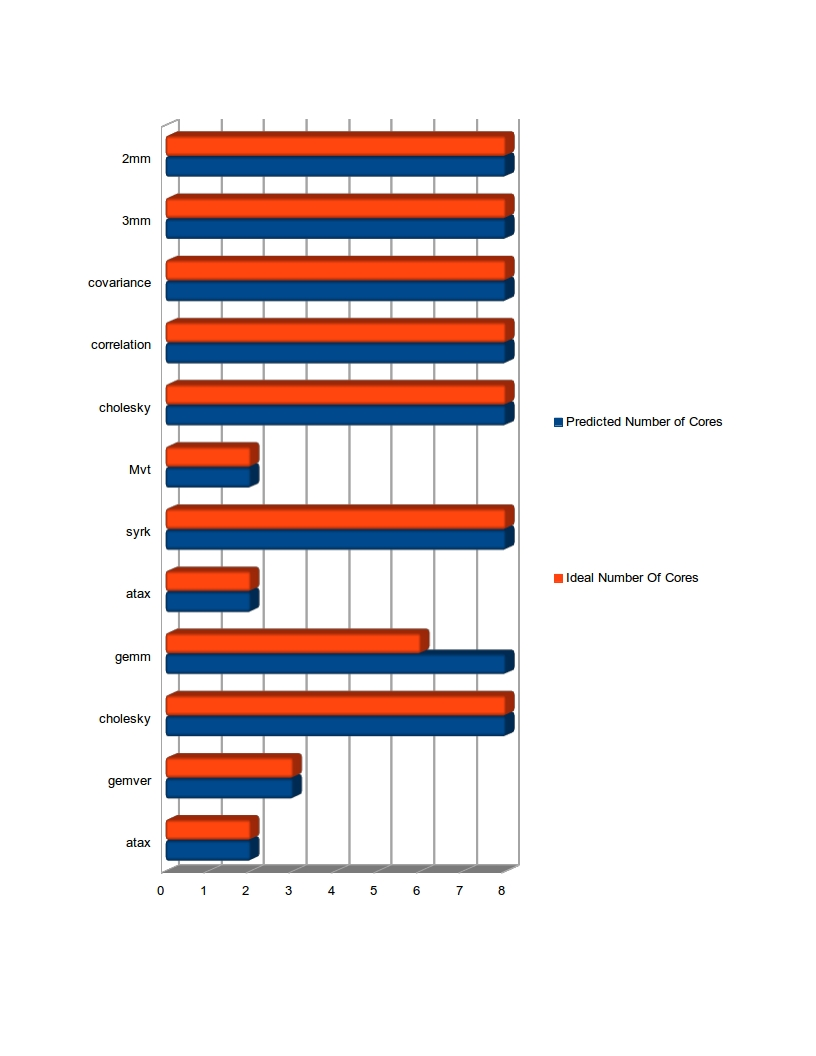
\includegraphics[width=160mm, height=180mm]{images/core-errors-C.jpg}
\caption{Deviation in predicted optimal number of cores for C applications \label{overflow}}
\end{center}
\end{figure}

\begin{figure}[ht!]
\begin{center}
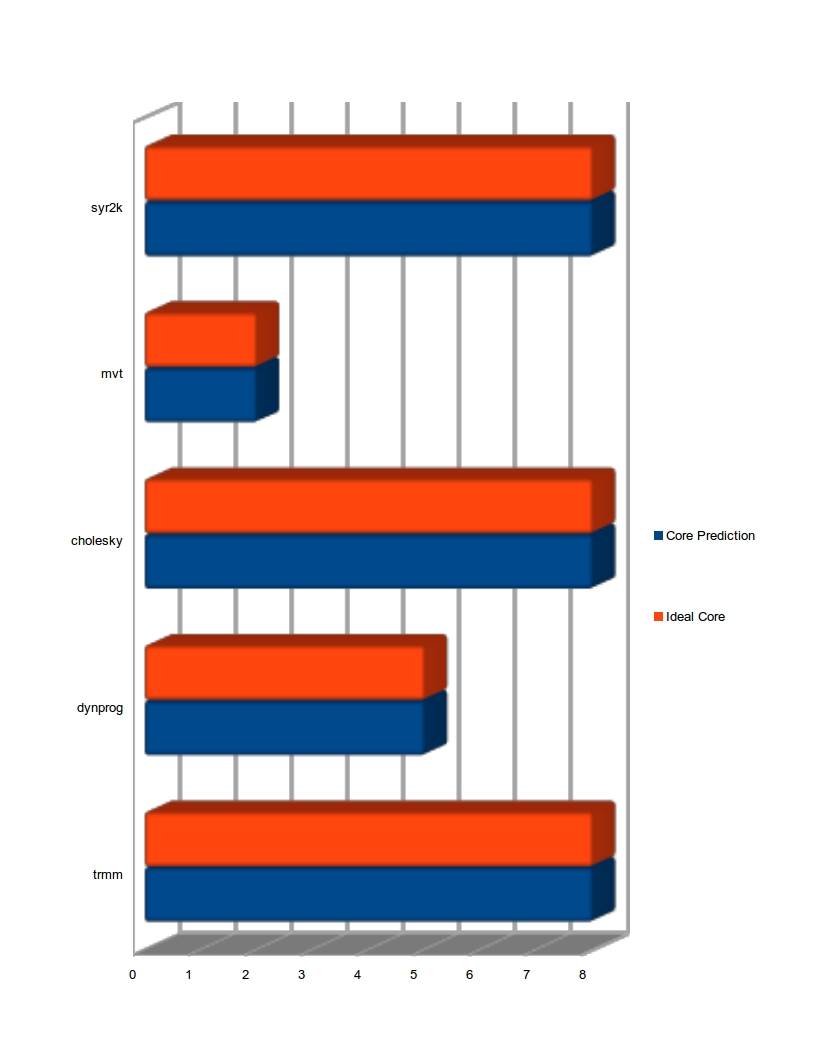
\includegraphics[width=160mm, height=180mm]{images/core-errors-LC.jpg}
\caption{Deviation in predicted optimal number of cores for LC applications \label{overflow}}
\end{center}
\end{figure}

\begin{figure}[ht!]
\begin{center}
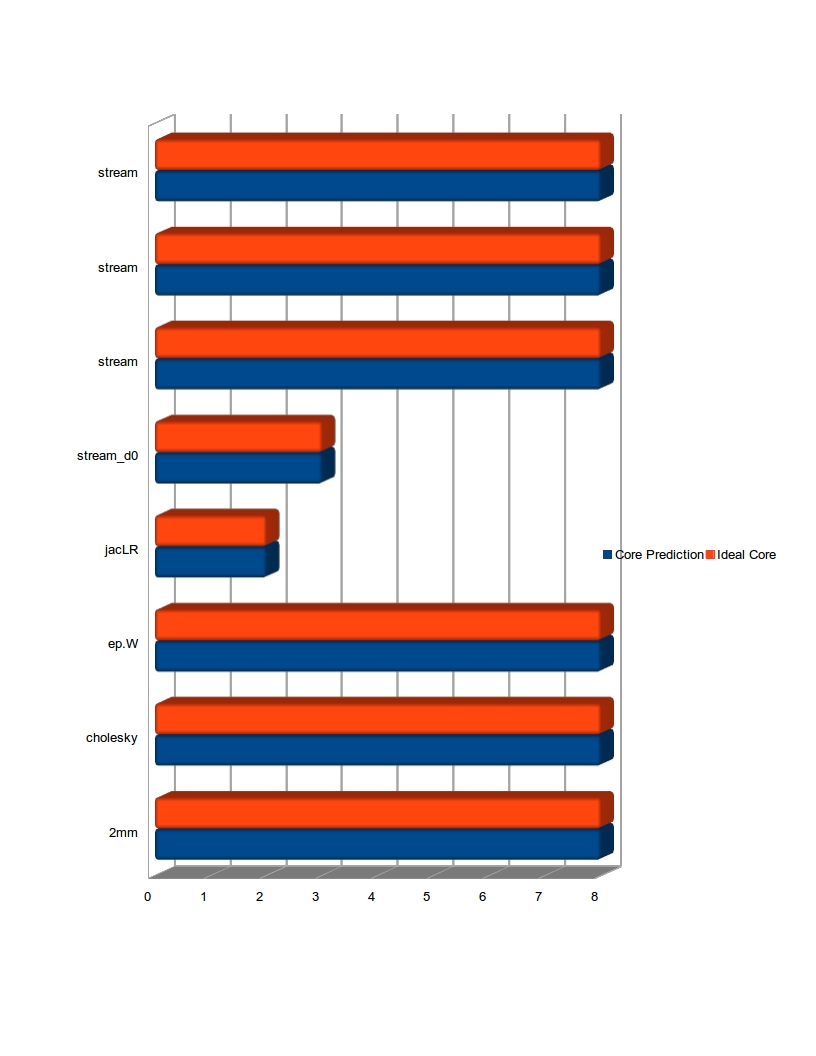
\includegraphics[width=160mm, height=180mm]{images/core-errors-LN.jpg}
\caption{Deviation in predicted optimal number of cores for L and N applications \label{overflow}}
\end{center}
\end{figure}

%\vspace{10mm}
\cleardoublepage

\section{Refinement}

We previously described that our prediction model provided specifically for applications L,C,C+ one relationship for each number of cores - 7 relationships in total - for each class of applications to predict the completion time that an application will have when allocated a specific number of cores. It was also proved that those relationships had low statistical errors in their predictions. However, for a more elegant and generic view, the prediction model can be transformed even more in order to reduce the number of those relationships. So, we examined this possibility and created a refined prediction model that contains a single prediction relationship for each class of applications that covers any number of cores. We also repeated the verification process in order to discover in what extent this tranformation affected the prediction errors. \\

The coefficients of the prediction model relationships follow a logarithmic trendline related to the number of cores. The correlation factors for this trendline proved to be over 0.95, which show a strong correlation. This correlation implies that we can extract a generic relationship from the multiple relations for each class of applications. We analysed the logarithmic trendline and the final generic relationships for the prediction model are the following (for classes L and C) : 

\begin{align*}
&Completion(LC)_{p}\ = \ [0.0139536*log(p)+0.0090562]*f_{LC}\ +\ [-0.252533*log(p)\ +\ 0.6407058] \ \\[3pt]
&Completion(C)_{p}\ = \ [0.2151318*log(p)+0.2239032]*f_{LC}\ +\ [-0.25468*log(p)\ +\ 0.6397947] \ \\[3pt]
&Ideal\_Completion_{p}\ =\ 1/p\\[3pt]
&R_{p}\ =\ (Ideal\_Completion_{p} / Completion_{p})*100\\[3pt]
&p_{optimum}\ =\  max\{p\},\ R_{p}\ >\ 70\\[3pt]
\end{align*}

To estimate the correctness of the refined generic prediction model, we compared the generic coefficients predicted by the logarithmic trendline with the original coefficients of the initial prediction model. In Figure 4.5 and 4.6, we can see the deviation from the original prediction model for class LC and class C of applications respectively.

\begin{figure}[ht!]
\begin{center}
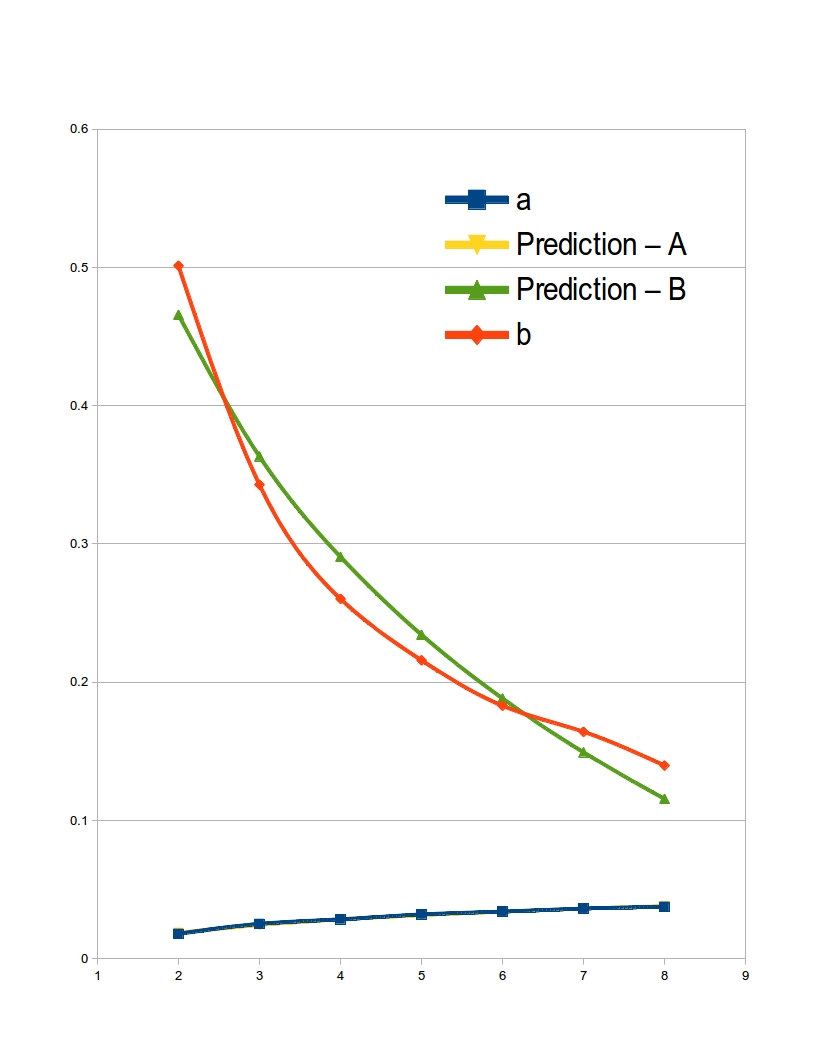
\includegraphics[width=160mm, height=180mm]{images/refined-prediction-LC.jpg}
\caption{Deviation for relationship $Completion(LC)_{p}=a*f_{LC}+b$ between initial and refined-predicted model \label{overflow}}
\end{center}
\end{figure}

\begin{figure}[ht!]
\begin{center}
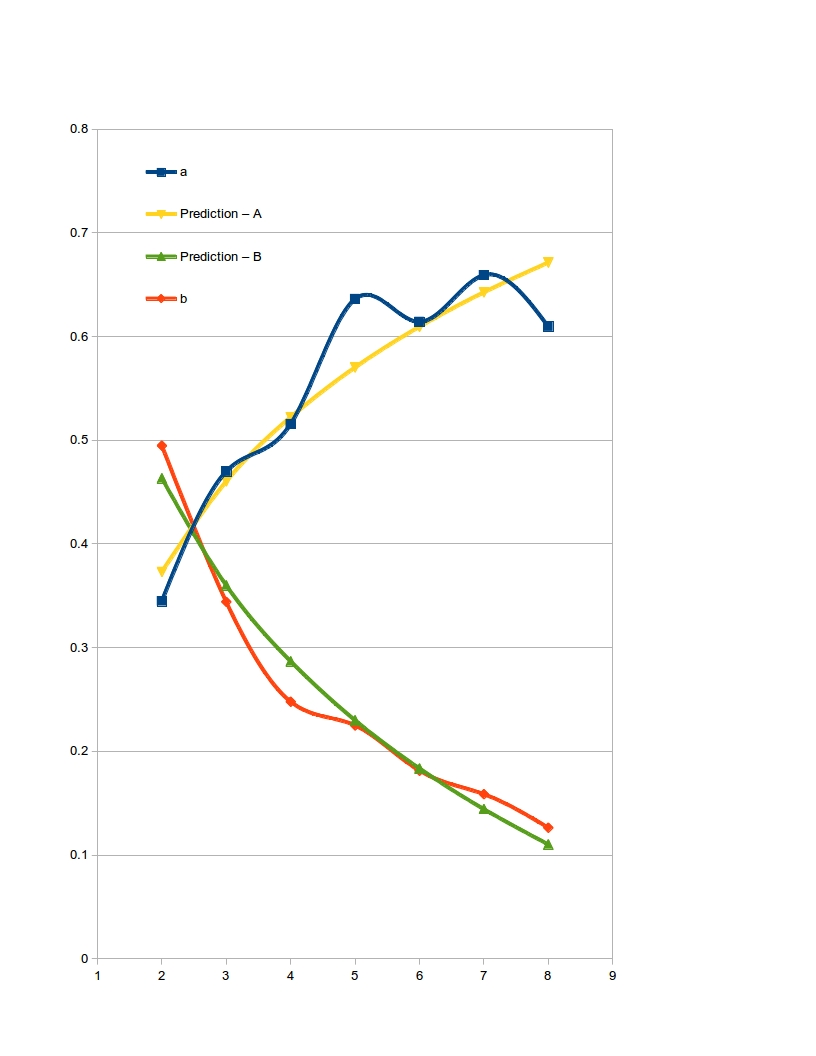
\includegraphics[width=160mm, height=180mm]{images/refined-prediction-C.jpg}
\caption{Deviation for relationship $Completion(C)_{p}=a*f_{C}+b$ between initial and refined-predicted model  \label{overflow}}
\end{center}
\end{figure}

\chapter{Scheduling}

The final step of the suggested scheduler is the algorithm used to co-schedule the applications. After having completed the first 2 steps for all the applications that need to be scheduled, each application is classified and the number of cores that should be allocated to it is defined. So, we can say that all applications are divided into 4 structures, each one containing the applications of a specific class along with the corresponding number of cores that will be allocated to each one. Then, the following algorithm is used to co-schedule the applications. We have made the realistic assumption that no more than 2 applications can be co-scheduled, so the algorithm attempts to co-schedule the applications solely in pairs. However, it can easily be extended to co-schedule using bigger combinations. \\

\section{Algorithm}

The algorithm uses 4 lists containing all the applications of each class and the optimal number of cores that should be allocated to each one. This algorithm iterates over each list of applications and for each application attempts to find a matching application (through method $popMatchFromTheEnd()$), so that the total number of allocated cores do not exceed the available cores of the current package. The function $coSchedule()$ increases, if possible, the cores of applications x and y equally, so that the sum is equal to the number of available cores of the system. Note that only for N-class applications, we select to allocate the half cores and schedule the applications 2 times, since their total performance will not degrade due to their cpu-bound profile. It is evident from the algorithm that some matches are attempted to be avoided, because the contention is aggravated. We need to avoid as much as possible the co-execution of L-C, L-L, L-LC pairs of applications, since the interference between the different sources of contention creates serious performance degradation. All the applications that will be left in the end of the algorithm, will execute with all the cores of the package allocated, so that there are no cores left idle. To take full advantage of the cores of the system, the lists of the applications are sorted with the applications requiring the least cores in the beginning and the function $popMatchFromTheEnd()$ searches all the lists given as parameters, starting from the end, to find one that can be co-scheduled with x. In this way, it is guaranteed that the cores that will be given in the end to the remaining applications will be the least possible.

\begin{Verbatim}[samepage=true, frame=single]
struct classifiedAndPredictedApplication{
    String name;
    int allocatedCores;
}; //sorted in ascending order by cores
classifiedAndPredictedApplication[] L,LC,C,N;

int main(){
    int initialSize = sizeof(N);
    for(i=0; i < initialSize; i++){
        N[i].allocatedCores = N[i].allocatedCores/2;
        N[initialSize+i] = N[i];
    }

    for(i=0; i < 2*initialSize; i++){                  
        x = N[i];
        y = x.popMatchFromTheEnd([C,L,LC,N]);
        if(y != null)  coSchedule(x,y);
    }
    for(i=0; i < sizeof(LC); i++){              
        x = LC[i];
        y = x.popMatchFromTheEnd([C,LC,L]);
        if(y != null)  coSchedule(x,y);
    }
    for(i=0; i < sizeof(L); i++){              
        x = L[i];
        y = x.popMatchFromTheEnd([L]);
        if(y != null)  coSchedule(x,y);
    }
    for(i=0; i < sizeof(C); i++){              
        x = C[i];
        y = x.popMatchFromTheEnd([C]);
        if(y != null)  coSchedule(x,y);
    }

    scheduleAllRemainingApplications();

return 1;
}


\end{Verbatim}

\small
\begin{Verbatim}[samepage=true, frame=single]
classifiedAndPredictedApplication 
    popMatchFromTheEnd(classifiedAndPredictedApplication[] processes){
        for(int i=0; i < sizeof(processes); i++){
            for(j=0; j < sizeof(processes[i]); j++){
                if( processes[i].allocatedCores + this.allocatedCores 
                                        < system.getPackageCores())
                    return processes[i];
            }
        }
    }

void 
    coSchedule(classifiedAndPredictedApplication a, 
                classifiedAndPredictedApplication b){
        while(a.allocatedCores+b.allocatedCores < system.getPackageCores()){
            a.allocatedCores++;
            if(a.allocatedCores+b.allocatedCores < system.getPackageCores())
                b.allocatedCores++;
        }
        system.schedule(a,b);
    }
\end{Verbatim}
\normalsize

\section{Comparison - Experimentation Results}

As analysed in the introductory chapter, we compared our proposed scheduler with the default Linux scheduler and with 2 more state-of-the-art contention-aware schedulers, LLC-MRB and LBB. For this comparison, a workload has been created with 17 applications from the Polyhedral Benchmark Suite \cite{reference8}, so that we have enough applications from all classes. The whole workload is executed for 1 hour, with quantums of 1 second, as stated before and when an application finishes, it gets respawned to execute again. Our scheduler is compared to LLC-MRB, LBB, the default Linux scheduler and a naive Gang scheduler in terms of fairness and total throughput. \\

The workload consisted of the following applications compiled in various sizes. In table, we can see the data sets for each application used : \\

\begin{table}[h]
\begin{center}
\caption{Benchmarks Data Sets}
\begin{tabular}{ | l | l | }
    \hline
    2mm & 1024 \\ \hline
    cholesky & 1024 \\ \hline
    jacobi & default suite large data set \\ \hline
    stream\_d0, stream\_d1 & 5*LLC cache size  \\ \hline
    trmm & 3000 \\ \hline
    dynprog & (700,350) \\ \hline
    mvt & 600 \\ \hline
    syr2k & 900 \\ \hline
    atax & 8000 \\ \hline
    gemver & 9000 \\ \hline
    gemm & 1150 \\ \hline
    cholesky & 4096 \\ \hline
    atax & 18000 \\ \hline
    correlation & 1500 \\ \hline
    covariance & 1500 \\ \hline
    2mm & 1500 \\ \hline
\end{tabular}
\end{center}
\end{table}


In the \textit{\textbf{Gang scheduler}}: all available cores (8) are allocated to each application and each application is executed alone. \\

In the \textit{\textbf{default Linux scheduler}}: the optimum number of cores as defined from the prediction model are allocated to each application and then the applications are left to be scheduled by CFS. This means that threads of the same applications might not be co-scheduled. \\

In \textit{\textbf{LLC-MRB}} and \textit{\textbf{LBB}}: the number of allocated cores for each application is defined by the prediction model, but applications are co-scheduled using a sorted list by LLC misses or memory bandwidth correspondingly and combining applications from the beginning of the list with applications from the end in order to balance the LLC misses and the memory bandwidth consumption correspondingly. Figure 5.1 gives a brief image of these scheduling algorithms.\\

\begin{figure}[ht!]
\begin{center}
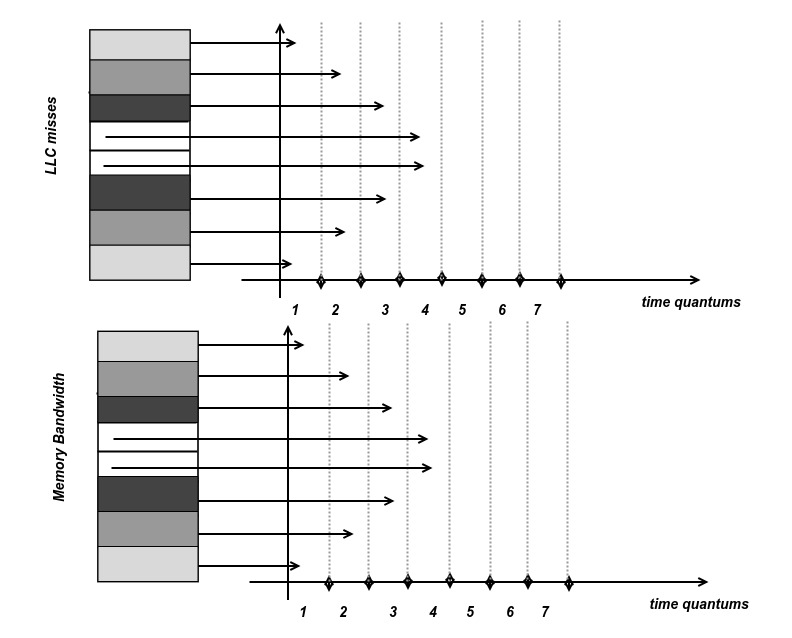
\includegraphics[width=150mm, height=120mm]{images/other_schedulers.jpg}
\caption{LLC-MRB and LBB balancing schedulers \label{overflow}}
\end{center}
\end{figure}

In our scheduler, called \textit{\textbf{LCN}}: the number of allocated cores are defined by the prediction model except from N applications, which are allocated the half cores and scheduled twice as described above. The workload is divided into pairs and alone applications using the previous algorithm. \\

In table 5.2, we can see the number of times each applications has been completed during the execution of the workload from the different schedulers. In the last rows of the table, we can also see the total number of executions of all the applications for each scheduler (corresponding to the the overall throughput of each scheduler), the number of most applications that each scheduler has achieved the best performance (a different measurement of overall throughput) and the standard deviation between the executions number of all applications for each scheduler (corresponding to the fairness). The schedulers can be compared in terms of overall throughput using 2 criterias : (i) the total number of times all the applications have been completed (ii) the total number of applications for which the scheduler has managed to achieve the biggest number of completions. The schedulers can also be compared in terms of fairness using the covariance between the completion-times number of each application and the corresponding completion-times number of the Gang scheduler. Green colour is used to point where a scheduler has managed to achieve the most completions for an application and yellow colour is used if there are multiple schedulers that have reached the maximum number. As it is evident, our scheduler outperforms CFS and the other state-of-the-art contention-aware schedulers in terms of overall throughput using both criteria. In terms of fairness, it seems that the other contention-aware schedulers are better with LLC-MRB being the best. However, this is not a clear conclusion, since it may not mean that some applications are unfairly treated by our scheduler, but instead that some applications are highly favoured by our scheduler. \\

%\hskip-0.15cm
\Large
\begin{table}[h]
\begin{center}
\caption{Comparison between schedulers}
\begin{tabular}{ | l | l | l | l | l | l | }
    \hline
    Benchmarks & Gang & CFS & LLC-MRB & LBB & LCN \\ \hline
    2mm & 54 & \cellcolor{yellow}101 & 92 & 92 & \cellcolor{yellow}101 \\ \hline
    cholesky & 55 & 124 & 92 & 92 & \cellcolor{green}136 \\ \hline
    jacobi & 13 & 15 & 13 & 16 & \cellcolor{green}17 \\ \hline
    stream\_d0 & 31 & 34 & 32 & 30 & \cellcolor{green}34 \\ \hline
    stream\_d1 & 31 & \cellcolor{green}34 & 21 & 32 & 21 \\ \hline
    trmm & 54 & \cellcolor{green}75 & 69 & 69 & 69 \\ \hline
    dynprog & 54 & 22 & 36 & \cellcolor{green}53 & 36 \\ \hline
    mvt & 43 & 31 & \cellcolor{green}39 & 34 & 30 \\ \hline
    syr2k & 72 & 80 & \cellcolor{yellow}92 & \cellcolor{yellow}92 & \cellcolor{yellow}92 \\ \hline
    atax & 27 & 20 & \cellcolor{green}25 & 19 & 22 \\ \hline
    gemver & 54 & 38 & \cellcolor{yellow}69 & \cellcolor{yellow}69 & 39 \\ \hline
    gemm & 72 & 85 & 55 & 55 & \cellcolor{green}92 \\ \hline
    cholesky & 43 & 49 & \cellcolor{yellow}55 & \cellcolor{yellow}55 & \cellcolor{yellow}55 \\ \hline
    atax & 43 & 25 & \cellcolor{green}46 & 21 & 39 \\ \hline
    correlation & 43 & \cellcolor{green}62 & 55 & 55 & 55 \\ \hline
    covariance & 43 & \cellcolor{green}62 & 55 & 55 & 55 \\ \hline
    2mm & 72 & 79 & 92 & 92 & 92 \\ \hline
    Total exec. & 804 & 936 & 938 & 931 & \cellcolor{green}985 \\ \hline
    Most Improved & - & 5 & 7 & 5 & \cellcolor{green}8 \\ \hline
    Standard Deviation & - & 0.46 & \cellcolor{green}0.30 & 0.32 & 0.46 \\ \hline
\end{tabular}
\end{center}
\end{table}

\normalsize

For a more qualitative view of the comparison between the different schedulers we can see the following graphs produced by table 5.2. First of all, we have calculated for each application and for each scheduler, the gain compared to the Gang scheduler by dividing with the corresponding executions number of the Gang scheduler. More formally, the calculations used the formula $cell_{i,j}=cell_{i,j}/cell_{i,1}, for \ i>=2$. Figure 5.2 presents the gains of the 4 schedulers compared separately per application. We have also calculated the average gain  and the standard deviation of gains for each scheduler. Figure 5.3 presents those results.

\begin{figure}[ht!]
\begin{center}
\hspace*{-3cm}
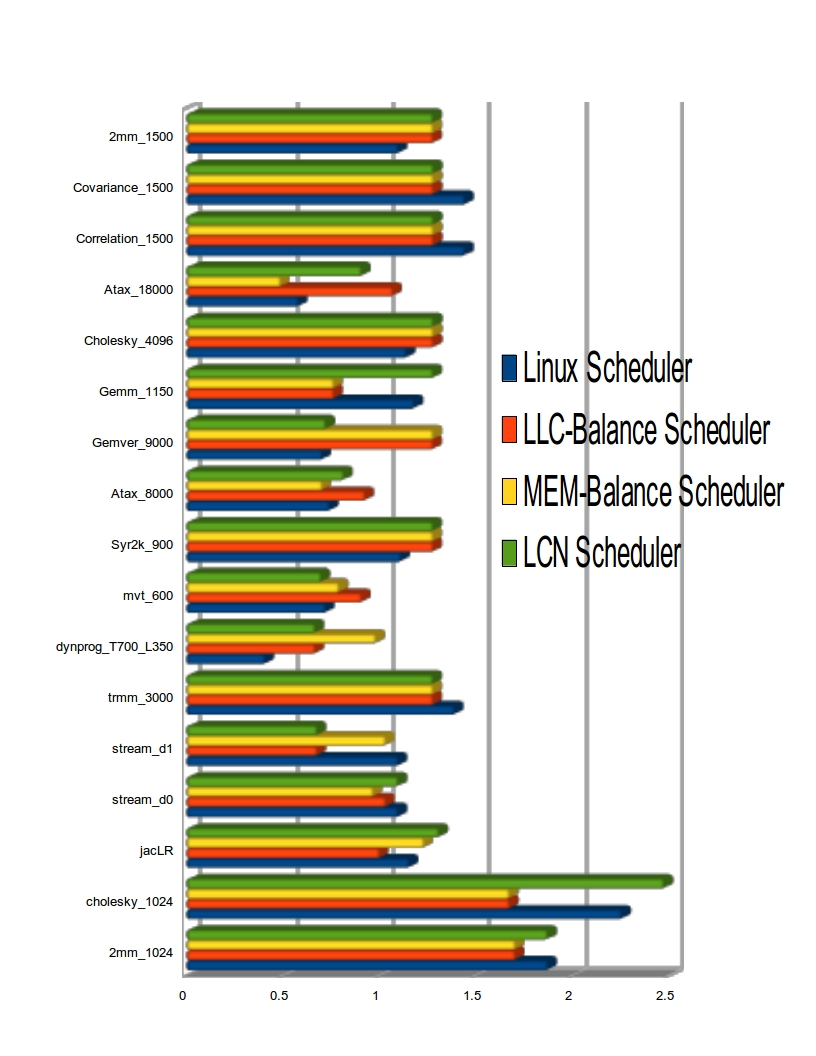
\includegraphics[width=200mm, height=200mm]{images/comparison.jpg}
\caption{Comparison of gains per application between 4 schedulers \label{overflow}}
\end{center}
\end{figure}

\begin{figure}[ht!]
\begin{center}
\hspace*{-3cm}
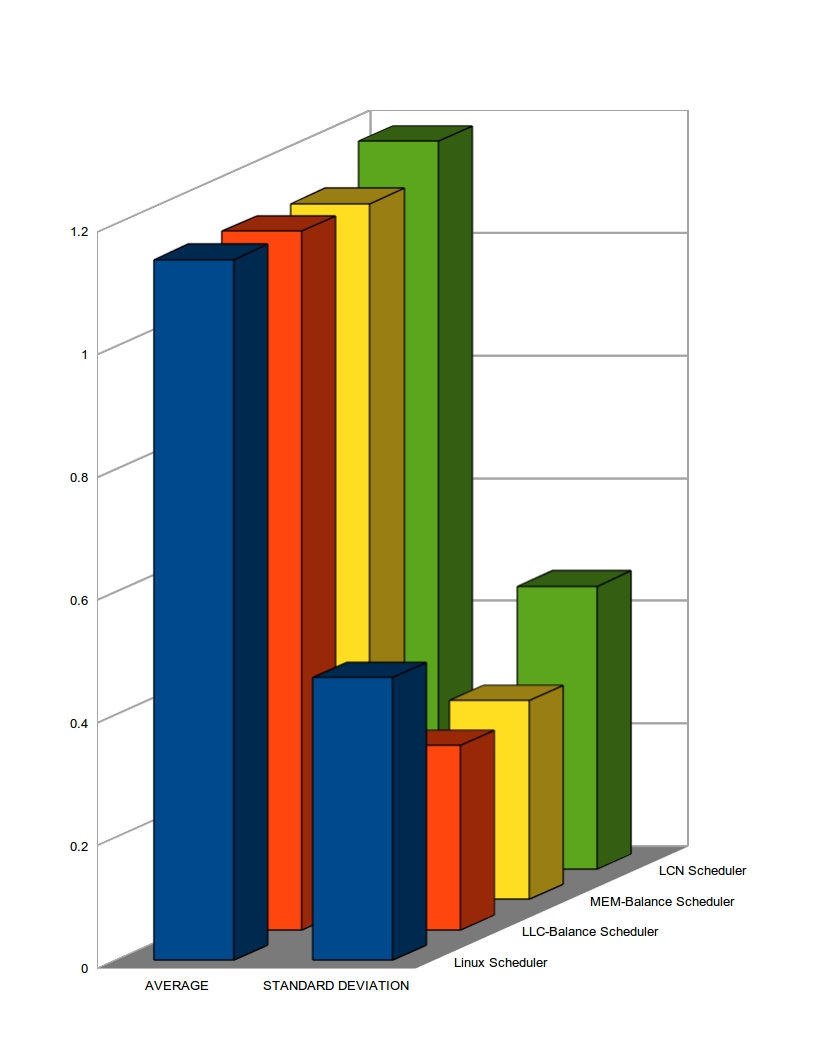
\includegraphics[width=200mm, height=200mm]{images/avg-stdev-comparison.jpg}
\caption{Comparison of average gain and standard deviation between 4 schedulers \label{overflow}}
\end{center}
\end{figure}

\cleardoublepage

Investigating the schedulers from a theoretic perspective, we can explain their difference in total throughput. \\

CFS scheduler, as described in the introduction, cannot take full advantage of multicore systems. CFS scheduler might even separate the same threads of an application to different time quantums. This will result in important parallelism gain losses. The data sharing patterns that would be otherwise leveraged will be ignored by CFS. Furthermore, being contention-unaware, CFS cannot locate resource contention and co-schedules threads in a contention-agnostic way, thus hurting significantly their performance. \\

On the other side, both LLC-MRB and LBB cannot differentiate between class N and C applications, since they both exhibit low LLC misses and memory link usage \cite{reference1}. As a result, they co-schedule class L applications with class C applications, thus creating even more contention. As it ws clarified in chapter 3, the co-execution of C and L applications results in dramatic slowdown of the C application. However, our scheduler can tell them apart through the classification scheme and limits the contention in a satisfying degree. This is simply the result of our classification scheme being directly bonded to the memory hierarchy of modern operating systems. \\

\chapter{Conclusion}

\section{General Remarks}

This thesis proposes a new contention-aware scheduler that is based on existing hardware infrastructure. The suggested scheduler does not require additional adjustments in modern operating systems. Due to its simplicity, it can easily be integrated as a subcomponent of the current scheduler or even constitute a novel independent scheduler. \\

Our proposed scheduler consists of 3 components : a classification scheme, a prediction model and a scheduling algorithm. The classification scheme is used to conduct a categorization of applications based on the part of the system resources, where they create contention. The classification scheme is also used to acquire a vision about the interference between applications belonging to different classes. The prediction model is used to estimate the optimum amount of resources that must be allocated to each application, so that the application achieves the best possible scaling proportionally to the resources allocated. This means that the prediction model is based on a compromise between application's scaling and resource management. The scheduling algorithm uses the first 2 components in order to derive the class of an application and define the optimum number of cores that shoulf be allocated to the application. Then, the algorithm takes the proper decisions in order to co-schedule the applications in a way that the overall performance of the system is maximised. \\

The scheduler presented in this thesis is compared to other state-of-the-art schedulers, like the default Linux scheduler (CFS), an LLC miss rate balancing scheduler (LLC-MRB) and a memory link balancing scheduler (LBB). The results of the experiments for the comparison between the different schedulers revealed that the proposed scheduler achieves the best overall performance in the system. It presents equal fairness to the Linux default scheduler and worse fairness than the other state-of-the-art schedulers. \\

The proposed scheduler can be incorporated in a real-life scheduling environment. To make this scenario feasible, 2 approaches can be followed. According to the first approach, each application that is inserted in the scheduling queue is initially executed for a really short period (around 2-3 quantums) to acquire the necessary HPC counters for the first 2 steps and then the application is re-inserted in the final queue classified and attached to its prediction. The other approach is to start scheduling the applications with minimal resources and dynamically monitor the HPC counter during the first quantums in order to dynamically adapt their resources afterwards. The dunamic adaptation of the scheduling is attainable, since the control group infrastructure can handle programs that create threads dynamically \cite{reference10}. After the classification and the definition of resource allocation for each application, the final scheduling algorithm is executed in the current queue to create the optimal combinations.\\

\section{Future Work}

This thesis was the starting point around this approach. Some of the improvements that could significantly ameliorate the results of this scheduler are the following :

\begin{itemize}
    \item Improvements in the prediction model. The prediction model can be re-designed using stepwise regression models. In this way, more variables can be added decreasing the statistical errors even more. However, we should not forget that there is a limitation regarding the number of hardware performance counters that can be simultaneously acquired during the execution of an application. So, on the one hand the addition of many variables in the prediction model would decrease the ease to integrate this scheduler in a real-life system. On the other hand, attention should be given to ensure that the added counters are not related by coincidence to the scaling of the application but it is a cause-effect relationship. Moreover, other methods can improve even more the credibility of our prediction model, such as machine learning.\\
    \item Extension of this scheduling approach to NUMA architectures. The suggested scheduling algorithm is implemented to function in NUMA architectures with only 1 package. However, it can be extended to multiple packages using thread migrations between different memory domains only when beneficial, since similar research has been conducted in the field of contention-aware thread migrations\cite{reference11}. Briefly, when investigating all the packages, we should try to allocate threads of the same application in the same package, which is possible as no application seemed to scale over the number of cores of a package for now.  So, threads migrations will be performed only when applications change drastically to a new class during the execution. On this occasion, thread migration will be performed alongside memory migration, so the total tradeoff should be taken into consideration. One important problem would arise in architectures with less cores in a package (such as the Nehalem arhictecture used with 4 cores per package), where the scheduling policy should be able to decide where threads of the same application would be positioned (if they will be time-scheduled or space-scheduled). \\
\end{itemize}


%%%  Bibliography

%\bibliographystyle{Styles/softlab-thesis}

\cleardoublepage
\phantomsection
\addcontentsline{toc}{chapter}{Bibliography}
%\bibliography{test}

\begin{thebibliography}{99}
\bibitem{reference1} A.Haritatos, G.Goumas, N.Anastopoulos, K.Nikas, K.Kourtis and N.Koziris. LCA: a memory link and cache-aware co-scheduling approach for CMPs. In Proceedings of the 23rd international conference on Parallel architectures and compilation, pages 469-470, 2010, ACM.
\bibitem{reference2} S.Blagodurov, S.Zhuravlev and A.Fedorova. Contention-Aware Scheduling on Multicore Systems. In ACM Transactions on Computer Systems (TOCS), 2010
\bibitem{reference3} Xiao Zhang, Sandhya Dwarkadas and Kai Shen. Towards practical page coloring-based multicore cache management. In Proceedings of the 4th ACM European conference on Computer systems, pages 89-102, 2009, ACM.
\bibitem{reference4} Moinuddin K. Qureshi and Yale N. Patt. Utility-Based Cache Partitioning: A Low-Overhead, High-Performance, Runtime Mechanism to Partition Shared Caches. In Proceedings of the 39th Annual IEEE/ACM International Symposium on Microarchitecture, pages 423-432, 2006, ACM.
\bibitem{reference5} Wm. A. Wulf and Sally McKee. Hitting the memory wall: implications of the obvious. In ACM SIGARCH Computer Architecture News, vol. 23, 1995, ACM.
\bibitem{reference6} E. Ebrahimi, O. Mutlu and Y. N. Patt. Techniques for bandwidth-efficient prefetching of linked data structures in hybrid prefetching systems. In IEEE 15th International Symposium on High Performance Computer Architecture, pages 7-17, 2009, IEEE.
\bibitem{reference7} Stream Benchmark, https://www.nersc.gov/users/computational-systems/cori/nersc-8-procurement/trinity-nersc-8-rfp/nersc-8-trinity-benchmarks/stream
\bibitem{reference8} The Polyhedral Benchmark suite, http://web.cse.ohio-state.edu/~pouchet/software/polybench
\bibitem{reference9} Intel Performance Counter Monitor - A better way to measure CPU utilization, http://software.intel.com/en-us/articles/intel-performance-counter-monitor
\bibitem{reference10} Cpusets: Processor and Memory Placement for Linux 2.6 kernel based systems, http://oss.sgi.com/projects/cpusets/
\bibitem{reference11} The freezer subsystem, https://www.kernel.org/doc/Documentation/cgroups/freezer-subsystem.txt
\bibitem{reference12} Kishore Kumar Pusukuri, David Vengerov, Alexandra Fedorova and Vana Kalogeraki. FACT: a framework for adaptive contention-aware thread migrations. In Proceedings of the 8th ACM International Conference on Computing Frontiers, 2011, ACM.
\bibitem{reference13} Major Bhadauria and Sally A. McKee. An approach to resource-aware co-scheduling for CMPs. In Proceedings of the 24th ACM International Conference on Supercomputing, ICS '10, pages 188-199, 2010, ACM.
\bibitem{reference14} Andreas Merkel, Jan Stoess and Frank Bellosa. Resource-conscious scheduling for energy efficiency on multicore processors. In Proceedings of the 5th European conference on Computer systems, EuroSys '10, pages 153-166, 2010, ACM.
\bibitem{reference15} Yuejian Xie and Gabriel Loh. Dynamic classification of program memory behaviors in CMPs. In Proceedings of the 2nd Workshop on Chip Multiprocessor Memory Systems and Interconnects, 2008.
\bibitem{reference16} Jiang Lin, Qingda Lu, Xiaoning Ding, Zhao Zhang, Xiaodong Zhang and P. Sadayappan. Gaining insights into multicore cache partitioning: Bridging the gap between simulation and real systems. In International Symposium on High Performance Computer Architecture, pages 367–378, 2008.
\bibitem{reference17} Chandandeep Singh Pabla. Completely fair scheduler. In Linux Journal, vol.2009, 2010.
\bibitem{reference18} G. E. Moore. Cramming More Components onto Integrated Circuits. In Proceedings of the IEEE, vol. 86, pages 82-85, 1998.
\bibitem{reference19} Allan Snavely and Dean M. Tullsen. Symbiotic jobscheduling for a simultaneous mutlithreading processor. In ACM SIGPLAN Notices, vol. 35, pages 234-244, 2000.
\bibitem{reference20} Alexandra Fedorova, Margo Seltzer and Michael D. Smith. Improving Performance Isolation on Chip Multiprocessors via an Operating System Scheduler. In PACT '07 Proceedings of the 16th International Conference on Parallel Architecture and Compilation Techniques, pages 25-38, 2007.
\bibitem{reference21} Knauerhase, R., Brett, P., Hohlt, B., Hahn, S.: Using OS Observations to Improve Performance in Multicore Systems. In: IEEE Micro 28, 3 , pp. 54-58 (2008).
\bibitem{reference22} Merkel, A., Stoess, J., Bellosa, F. : Resource-Conscious Scheduling for Energy Efficiency on Multicore Processors. In: Proceedings of EuroSys, pp.6-8, pp.11-13 (2010).
\bibitem{reference23} Zhuravlev, S., Blagodurov, S., Fedorova, A.: Addressing Contention on Multicore Processors via Scheduling. In: Proceedings of ASPLOS, pp.1-6 (2010).
\bibitem{reference24} Li, T., Baumberger, D., Koufaty, D.A., Hahn, S.: Efficient Operating System Scheduling for Performance-Asymmetric Multi-core Architectures. In: Proceedings of Supercomputing, pp.1-4, pp.8-10 (2007).


\end{thebibliography}
%%%  End of document

\end{document}
